\documentclass[11pt,a4paper]{article}
\usepackage{fontspec}
% Liberation Sans tem as medidas da Arial; sem ela, usa a TeX Gyre Heros
\IfFontExistsTF{Liberation Sans}{\setmainfont{Liberation Sans}}{\setmainfont{TeX Gyre Heros}}
\IfFontExistsTF{Liberation Mono}{\setmonofont{Liberation Mono}}{\setmonofont{TeX Gyre Cursor}}
\usepackage{polyglossia}
\setdefaultlanguage[variant=brazilian]{portuguese}
\usepackage[left=3cm,right=2cm,top=3cm,bottom=2cm,headsep=0.8cm]{geometry}
\usepackage{setspace}
\setstretch{1.35}
\setlength{\parindent}{0pt}
\setlength{\emergencystretch}{2.5em}
\setlength{\parskip}{6pt plus 1pt}
\usepackage{graphicx}
\usepackage[table]{xcolor}
\usepackage{array,booktabs,tabularx,multirow,makecell}
\usepackage{fancyhdr}
\usepackage{titlesec}
\usepackage{tocloft}
\usepackage{caption}
\usepackage{float}
\usepackage[section,above]{placeins}
\usepackage{flafter}
\usepackage{fancyvrb}
\usepackage{multicol}
\setlength{\columnsep}{0.8cm}
\usepackage{amsmath}
\usepackage{tikz}
\usetikzlibrary{positioning,calc,arrows.meta,fit,backgrounds,shapes.geometric,decorations.pathreplacing}
\usepackage[hidelinks]{hyperref}
\usepackage{xurl}
\urlstyle{same}
\hypersetup{pdftitle={Lab de configuração básica de rede com VLANs e VLSM},
  pdfauthor={Gabriel André de Lima Silva},
  pdfsubject={Atividade de Redes I, Professor Fred Sauer}}

\definecolor{hostblue}{HTML}{2F5DA8}
\definecolor{vprof}{HTML}{1F5FAD}
\definecolor{valun}{HTML}{2E7D32}
\definecolor{vvisi}{HTML}{B85C00}
\definecolor{gridgray}{gray}{0.72}
\newcommand{\hb}[1]{\textcolor{hostblue}{#1}}

% cabecalho: numero da pagina no canto superior direito
\pagestyle{fancy}
\fancyhf{}
\fancyhead[R]{\small\thepage}
\renewcommand{\headrulewidth}{0pt}

% titulos
\titleformat{\section}{\normalfont\bfseries}{}{0pt}{}
\titleformat{\subsection}{\normalfont\bfseries}{}{0pt}{}
\titleformat{\subsubsection}{\normalfont\bfseries}{}{0pt}{}
\titlespacing*{\section}{0pt}{14pt}{6pt}
\titlespacing*{\subsection}{0pt}{10pt}{4pt}
\titlespacing*{\subsubsection}{0pt}{8pt}{2pt}
\newcommand{\secao}[1]{\section*{#1}\phantomsection\addcontentsline{toc}{section}{#1}}
\newcommand{\subsecao}[1]{\subsection*{#1}\phantomsection\addcontentsline{toc}{subsection}{#1}}

% sumario
\renewcommand{\cfttoctitlefont}{\hfill\normalsize\bfseries}
\renewcommand{\cftaftertoctitle}{\hfill}
\setlength{\cftbeforetoctitleskip}{0pt}
\setlength{\cftaftertoctitleskip}{14pt}
\renewcommand{\cftsecfont}{\small\bfseries}
\renewcommand{\cftsecpagefont}{\small\bfseries}
\renewcommand{\cftsubsecfont}{\small}
\renewcommand{\cftsubsecpagefont}{\small}
\renewcommand{\cftsecleader}{\bfseries\cftdotfill{\cftdotsep}}
\setlength{\cftbeforesecskip}{2pt}
\setlength{\cftsubsecindent}{1.2em}
\setlength{\cftsecindent}{0pt}

% legendas: "Tabela 1: ..." acima, fonte embaixo
\captionsetup{font=small,labelsep=colon,justification=raggedright,singlelinecheck=false,skip=3pt}
\captionsetup[table]{position=top}
\newcommand{\fonte}{\par\vspace{1pt}{\small Fonte: elaborado pelo autor.}\par}
\newcommand{\fontebase}[1]{\par\vspace{1pt}{\small Fonte: elaborado pelo autor com base em #1.}\par}
\newcommand{\fonteprint}{\par\vspace{1pt}{\small Fonte: captura de tela do Cisco Packet Tracer feita pelo autor.}\par}
\newcommand{\fonteadapt}{\par\vspace{1pt}{\small Fonte: adaptado de Sauer ([\emph{s. d.}]a).}\par}

% tabela de contas em binario (grade cinza, cabecalho sombreado)
\newenvironment{bintab}{%
  \par\vspace{2pt}\noindent\begingroup\small\arrayrulecolor{gridgray}\renewcommand{\arraystretch}{1.25}%
  \begin{tabular}{|l|l|l|}\hline
  \rowcolor{gray!14} & \multicolumn{1}{c|}{\bfseries Binário (rede | host)} & \multicolumn{1}{c|}{\bfseries Decimal}\\ \hline}
 {\end{tabular}\endgroup\par\vspace{6pt}}
\newenvironment{andtab}{%
  \par\vspace{2pt}\noindent\begingroup\small\renewcommand{\arraystretch}{1.15}\begin{tabular}{@{}l@{\hspace{1em}}l@{\hspace{1em}}l@{}}}
 {\end{tabular}\endgroup\par\vspace{6pt}}
\newenvironment{somatab}{%
  \par\vspace{2pt}\noindent\begingroup\small\renewcommand{\arraystretch}{1.15}\begin{tabular}{@{}l@{\hspace{0.6em}}r@{\hspace{1em}}l@{}}}
 {\end{tabular}\endgroup\par\vspace{6pt}}

% blocos de comandos
\DefineVerbatimEnvironment{cmd}{Verbatim}{fontsize=\small,xleftmargin=1.2em,frame=leftline,framerule=0.6pt,rulecolor=\color{gray!60},framesep=8pt,samepage=true,baselinestretch=1.08}
\DefineVerbatimEnvironment{conf}{Verbatim}{fontsize=\scriptsize,baselinestretch=1.0}
\DefineVerbatimEnvironment{saida}{Verbatim}{fontsize=\footnotesize,xleftmargin=0.4em,frame=single,rulecolor=\color{gray!50},framesep=6pt,samepage=true,baselinestretch=1.0}

\newcolumntype{C}[1]{>{\centering\arraybackslash}p{#1}}
\setlength{\cftfigindent}{0pt}

% icones e estilos comuns aos diagramas
\tikzset{
  sw/.pic={\draw[fill=white, rounded corners=2pt] (-0.55,-0.22) rectangle (0.55,0.22);
           \draw[-{Stealth[length=3pt]}] (-0.32,0.07) -- (0.32,0.07);
           \draw[-{Stealth[length=3pt]}] (0.32,-0.07) -- (-0.32,-0.07);},
  rt/.pic={\draw[fill=white] (0,0) circle (0.36);
           \draw[{Stealth[length=3pt]}-{Stealth[length=3pt]}] (-0.22,-0.22) -- (0.22,0.22);
           \draw[{Stealth[length=3pt]}-{Stealth[length=3pt]}] (-0.22,0.22) -- (0.22,-0.22);},
  pc/.pic={\draw[fill=white, rounded corners=1pt] (-0.32,-0.12) rectangle (0.32,0.30);
           \draw (0,-0.12) -- (0,-0.22); \draw (-0.16,-0.24) -- (0.16,-0.24);},
  porta/.style={font=\scriptsize, text=black!80, fill=white, inner sep=0.6pt},
  info/.style={draw, rounded corners=1.5pt, align=left, font=\scriptsize, inner sep=3pt,
               line width=0.6pt, text width=2.65cm},
}
% tronco 802.1Q: tres linhas paralelas, uma por VLAN
\newcommand{\tronco}[2]{%
  \draw[vvisi, line width=0.9pt] ($(#1)!1.8pt!90:(#2)$) -- ($(#2)!1.8pt!-90:(#1)$);
  \draw[valun, line width=0.9pt] (#1) -- (#2);
  \draw[vprof, line width=0.9pt] ($(#1)!1.8pt!-90:(#2)$) -- ($(#2)!1.8pt!90:(#1)$);}

% listas de figuras e de tabelas
\tocloftpagestyle{empty}
\renewcommand{\cftloftitlefont}{\hfill\normalsize\bfseries}
\renewcommand{\cftafterloftitle}{\hfill}
\renewcommand{\cftlottitlefont}{\hfill\normalsize\bfseries}
\renewcommand{\cftafterlottitle}{\hfill}
\setlength{\cftbeforeloftitleskip}{0pt}
\setlength{\cftafterloftitleskip}{14pt}
\setlength{\cftbeforelottitleskip}{0pt}
\setlength{\cftafterlottitleskip}{14pt}
\renewcommand{\cftfigpresnum}{Figura~}
\renewcommand{\cftfigaftersnum}{:}
\setlength{\cftfignumwidth}{5.6em}
\renewcommand{\cfttabpresnum}{Tabela~}
\renewcommand{\cfttabaftersnum}{:}
\setlength{\cfttabnumwidth}{5.6em}
\setlength{\cftbeforefigskip}{3pt}
\setlength{\cftbeforetabskip}{3pt}


\begin{document}
\hyphenation{TANENBAUM WETHERALL KUROSE PLUMMER POSTEL SAUER REKHTER PUMMILL MANNING MOGUL FULLER CISCO SYSTEMS}
\renewcommand{\contentsname}{SUMÁRIO}
\renewcommand{\listfigurename}{LISTA DE FIGURAS}
\renewcommand{\listtablename}{LISTA DE TABELAS}

% =================================================================== CAPA
\begin{titlepage}
\thispagestyle{empty}
\centering
\vspace*{-1.2cm}

\includegraphics[width=3.55cm]{logo_uerj.pdf}\par
\vspace{1.1cm}
{\bfseries UNIVERSIDADE DO ESTADO DO RIO DE JANEIRO\par\vspace{0.25cm}
CAMPUS ZONA OESTE (UERJ-ZO)\par\vspace{0.25cm}
CURSO DE CIÊNCIA DA COMPUTAÇÃO\par}
\vspace{3.6cm}
GABRIEL ANDRÉ DE LIMA SILVA\par
\vspace{3.6cm}
{\Large\bfseries LAB DE CONFIGURAÇÃO BÁSICA DE REDE\\[2pt] COM VLANS E VLSM\par}
\vspace{0.45cm}
Endereçamento VLSM, VLANs, troncos 802.1Q e roteamento\\ router on a stick no Packet Tracer\par
\vspace{1.4cm}
\hspace*{6.8cm}\begin{minipage}{6.5cm}\small\raggedright
Atividade Pontuada de Redes I\\[4pt]
Professor: Fred Sauer
\end{minipage}
\vfill
{\bfseries RIO DE JANEIRO\par\vspace{0.25cm}2026\par}
\end{titlepage}

% ===================================================== LISTAS E SUMARIO
\setcounter{page}{2}
\begingroup
\setstretch{1.0}\setlength{\parskip}{0pt}
\listoffigures
\clearpage
\listoftables
\clearpage
\tableofcontents
\endgroup
\clearpage

% ============================================================== INTRODUCAO
\secao{INTRODUÇÃO}

Este relatório documenta a montagem do \emph{Lab de configuração básica de rede com VLANs e VLSM} (SAUER, [2023?]) no Cisco Packet Tracer. O cenário é um ambiente educacional com três grupos de usuários, cada um em uma VLAN: Professor (VLAN 10) com 60 pontos de rede, Alunos (VLAN 20) com 200 pontos e Visita (VLAN 30) com 500 pontos. A topologia tem três switches 2960 (SW1, SW2 e SW3), um roteador ISR 4331 e seis PCs, dois de cada VLAN.

O objetivo é definir a melhor distribuição de endereços privados para as três VLANs, separar os grupos em VLANs nos switches e permitir a comunicação entre elas por meio do roteador, com a técnica \emph{router on a stick}. O relatório apresenta os cálculos do endereçamento em binário, os comandos usados em cada equipamento e os testes que mostram o funcionamento da rede. O arquivo do Packet Tracer (.pkt) foi entregue junto com este documento e já está com todas as configurações salvas.

% ============================================================ FUNDAMENTACAO
\secao{FUNDAMENTAÇÃO}

\subsecao{VLAN e domínio de broadcast}

Um switch sem VLAN forma um único domínio de broadcast: um quadro enviado para o endereço FF:FF:FF:FF:FF:FF sai por todas as portas, exceto a de entrada. A VLAN divide o switch em redes locais lógicas. Um quadro que entra em uma porta da VLAN 10 só sai por portas que também são da VLAN 10, de modo que o broadcast fica restrito ao grupo (TANENBAUM; WETHERALL, 2011, seção 4.8.5; SAUER, [s. d.]b). Como cada VLAN é uma rede separada, ela recebe uma subrede IP própria, e o tráfego entre VLANs diferentes precisa passar por um roteador.

\subsecao{Tabela CAM e aprendizado do switch}

O switch decide por qual porta encaminhar cada quadro consultando a sua tabela CAM, que associa endereço MAC, VLAN e porta. Essa tabela é preenchida automaticamente, por aprendizado: quando um quadro chega, o switch anota o MAC de origem, a VLAN e a porta por onde ele entrou (TANENBAUM; WETHERALL, 2011, seção 4.8.2; KUROSE; ROSS, 2021, cap. 6). Se o MAC de destino já está na tabela, o quadro sai só pela porta anotada. Se não está, ou se o destino é o broadcast, o quadro é inundado por todas as portas da mesma VLAN, menos a de entrada. Como a tabela é separada por VLAN, o mesmo MAC pode aparecer em mais de uma VLAN, o que acontece com o MAC do roteador neste laboratório.

As entradas expiram depois de um tempo sem uso, 300 segundos por padrão nos switches Cisco (CISCO SYSTEMS, [s. d.]a). O roteiro pede que o cenário seja reiniciado antes do teste para esvaziar as tabelas CAM. O reinício também esvazia as tabelas ARP, e assim o modo simulação mostra toda a troca de mensagens desde a primeira pergunta ARP.

\subsecao{Porta de acesso e tronco 802.1Q}

A porta de acesso pertence a uma única VLAN e trabalha com quadros Ethernet comuns, sem marcação. É nela que ficam os PCs, que enviam e recebem quadros sem tag e não precisam saber a qual VLAN pertencem. O tronco é o enlace que transporta várias VLANs ao mesmo tempo, como os enlaces entre os switches e entre o SW3 e o roteador. Para o equipamento do outro lado saber de qual VLAN veio cada quadro, o padrão IEEE 802.1Q insere uma marca (\emph{tag}) de 4 bytes logo depois do MAC de origem (IEEE, 2018; TANENBAUM; WETHERALL, 2011, seção 4.8.5), como mostra a Figura~\ref{fig:quadro}.

\begin{figure}[H]
\captionsetup{position=top}
\caption{quadro Ethernet com a tag 802.1Q}\label{fig:quadro}
\centering
\begin{tikzpicture}[every node/.append style={execute at begin node=\setstretch{1.05}}, font=\small,
  campo/.style={draw, minimum height=0.95cm, align=center, inner sep=2pt, text height=1.7ex, text depth=0.45ex},
  tam/.style={font=\footnotesize, text=black!65},
  bits/.style={font=\footnotesize\ttfamily, text=hostblue}]
  % quadro Ethernet com tag
  \node[campo, minimum width=2.3cm] (dst) at (1.15,0) {Destino};
  \node[campo, minimum width=2.3cm, right=0pt of dst] (src) {Origem};
  \node[campo, minimum width=2.5cm, right=0pt of src, fill=hostblue!15, very thick] (tag) {Tag 802.1Q};
  \node[campo, minimum width=1.7cm, right=0pt of tag] (tipo) {Tipo};
  \node[campo, minimum width=4.2cm, right=0pt of tipo] (dados) {Dados};
  \node[campo, minimum width=1.6cm, right=0pt of dados] (fcs) {FCS};
  \foreach \n/\t in {dst/6 bytes, src/6 bytes, tag/4 bytes, tipo/2 bytes, dados/46 a 1500 bytes, fcs/4 bytes}
    \node[tam, above=1pt of \n] {\t};
  % detalhe dos 4 bytes da tag
  \node[campo, minimum width=4.4cm, anchor=north west] (tpid) at ($(dst.south west)+(1.0,-1.55)$) {TPID};
  \node[campo, minimum width=1.4cm, right=0pt of tpid] (pcp) {PCP};
  \node[campo, minimum width=1.1cm, right=0pt of pcp] (dei) {DEI};
  \node[campo, minimum width=4.6cm, right=0pt of dei, fill=hostblue!15] (vid) {VID (número da VLAN)};
  \draw[gray] (tag.south west) -- (tpid.north west);
  \draw[gray] (tag.south east) -- (vid.north east);
  \draw[decorate, decoration={brace, amplitude=4pt}, black!60] ($(pcp.north west)+(0,0.08)$) -- node[above=3pt, tam] {TCI: 16 bits} ($(vid.north east)+(0,0.08)$);
  % bits do exemplo: quadro da VLAN 10
  \node[bits, below=3pt of tpid] (b1) {1000 0001 0000 0000};
  \node[bits, below=3pt of pcp] {000};
  \node[bits, below=3pt of dei] {0};
  \node[bits, below=3pt of vid] (b4) {0000 0000 1010};
  \node[tam, below=1pt of b1] {16 bits = 0x8100};
  \node[tam] at (pcp |- b1.south) [below=1pt] {3 bits};
  \node[tam] at (dei |- b1.south) [below=1pt] {1 bit};
  \node[tam, below=1pt of b4] {12 bits = 10};
  \node[font=\footnotesize, anchor=east, align=right, text=hostblue] at ($(tpid.west |- b1)+(-0.15,0)$) {exemplo:\\VLAN 10};
\end{tikzpicture}

\fontebase{IEEE (2018) e Tanenbaum e Wetherall (2011)}
\end{figure}

O TPID vale 0x8100 e ocupa a posição em que um quadro comum teria o campo Tipo. É assim que o equipamento percebe que o quadro tem tag; o Tipo verdadeiro (0x0800 para IPv4, 0x0806 para ARP) vem logo depois da tag. Nos 2 bytes seguintes, chamados de TCI, ficam a prioridade (PCP, 3 bits), o bit DEI e o identificador da VLAN (VID, 12 bits). Com 12 bits é possível representar 2\textsuperscript{12} = 4096 valores, mas o 0 e o 4095 são reservados, por isso os números válidos de VLAN vão de 1 a 4094, o mesmo intervalo que aparece no roteiro para o \texttt{show vlan id}.

A parte de baixo da Figura~\ref{fig:quadro} mostra os bits de um quadro da VLAN 10: 10 = 8 + 2 = 1010, que ocupa o fim dos 12 bits do VID. Nas outras VLANs do laboratório o VID fica 0000 0001 0100 (20 = 16 + 4) e 0000 0001 1110 (30 = 16 + 8 + 4 + 2). Como a tag muda o conteúdo do quadro, o FCS é recalculado, e o tamanho máximo do quadro passa de 1518 para 1522 bytes.

Os quadros da VLAN nativa atravessam o tronco sem tag. No equipamento Cisco a VLAN nativa padrão é a 1, e o roteiro pede que ela não seja alterada (SAUER, [2023?]). O comando \texttt{switchport trunk allowed vlan 10,20,30} limita o tronco às três VLANs do cenário, já que por padrão o tronco aceita todas (CISCO SYSTEMS, [s. d.]d).

\subsecao{Roteamento entre VLANs com router on a stick}

Na técnica \emph{router on a stick} o roteador usa uma única interface física ligada a uma porta de tronco do switch. Essa interface é dividida em subinterfaces, uma por VLAN. Cada subinterface recebe o comando \texttt{encapsulation dot1Q} com o número da VLAN e o endereço IP que vai ser o gateway daquela VLAN (CISCO SYSTEMS, [s. d.]b). Quando chega um quadro com tag 10, ele é entregue à subinterface G0/0/0.10. Quando o roteador envia um pacote para a VLAN 20, o quadro sai pela G0/0/0.20 com tag 20. Para o roteador, cada subinterface é uma interface comum ligada a uma rede diferente, como mostra a visão lógica da Figura~\ref{fig:logica}, na seção 2.1.

O mesmo cabo leva o pacote duas vezes, na ida até o roteador e na volta para o switch. Essa é a principal limitação da técnica quando o tráfego entre VLANs é grande. O roteiro lembra que a comunicação entre VLANs também poderia ser feita com interfaces separadas de um roteador ou com um switch de camada 3, mas essas alternativas ficam fora do escopo deste laboratório (SAUER, [2023?]).

\subsecao{ARP e o papel do gateway}

Antes de enviar um pacote, o host faz o AND entre o IP de destino e a sua própria máscara. Se o resultado for igual ao endereço da sua rede, o destino está na mesma subrede e o host pergunta via ARP o MAC do próprio destino. Se for diferente, o pacote vai para o gateway, e o ARP pergunta o MAC do gateway. A pergunta do ARP é um broadcast e a resposta é unicast (PLUMMER, 1982; TANENBAUM; WETHERALL, 2011, seção 5.6.4). Com VLANs esse broadcast só chega aos equipamentos da mesma VLAN, e é essa redução de broadcast que o roteiro pede para observar no modo simulação. A Figura~\ref{fig:decisao} resume a decisão do host.

\begin{figure}[H]
\captionsetup{position=top}
\caption{decisão do host antes de enviar um pacote}\label{fig:decisao}
\centering
\begin{tikzpicture}[every node/.append style={execute at begin node=\setstretch{1.05}}, font=\small, x=1cm, y=1cm,
  passo/.style={draw, rounded corners=2pt, align=center, inner sep=4pt, text width=5.0cm, fill=white, minimum height=0.9cm},
  decisao/.style={draw, diamond, aspect=2.8, align=center, inner sep=0pt, text width=2.9cm, fill=white},
  ex/.style={font=\footnotesize, text=black!60, align=center, text width=5.0cm},
  seta/.style={-{Stealth[length=5pt]}, thick}]
  \node[passo] (ini) at (0,0) {o PC tem um pacote para um IP de destino};
  \node[passo] (and) at (0,-1.35) {AND entre o IP de destino e a máscara do próprio PC};
  \node[decisao] (dec) at (0,-3.05) {o resultado é a rede do próprio PC?};
  \node[passo, fill=valun!8] (arpd) at (-3.6,-4.75) {ARP pelo IP do \textbf{destino}};
  \node[passo, fill=hostblue!8] (arpg) at (3.6,-4.75) {ARP pelo IP do \textbf{gateway}};
  \node[passo] (envd) at (-3.6,-6.15) {quadro vai direto para o MAC do destino, sem passar pelo roteador};
  \node[passo] (envg) at (3.6,-6.15) {quadro vai para o MAC do gateway; o IP de destino não muda};
  \node[ex, below=3pt of envd] {exemplo: PC1 para PC4\\(o AND resulta em 192.168.3.0, a rede do PC1)};
  \node[ex, below=3pt of envg] {exemplo: PC1 para PC5\\(o AND resulta em 192.168.2.0, outra rede)};
  \draw[seta] (ini) -- (and);
  \draw[seta] (and) -- (dec);
  \draw[seta] (dec.west) -| node[above, pos=0.35] {sim} (arpd.north);
  \draw[seta] (dec.east) -| node[above, pos=0.35] {não} (arpg.north);
  \draw[seta] (arpd) -- (envd);
  \draw[seta] (arpg) -- (envg);
\end{tikzpicture}

\fontebase{Plummer (1982) e Tanenbaum e Wetherall (2011)}
\end{figure}

Depois da primeira resposta, o mapeamento fica guardado na tabela ARP do host, e as mensagens seguintes não precisam perguntar de novo. Além disso, quem recebe uma pergunta ARP dirigida a si já guarda o MAC de quem perguntou (PLUMMER, 1982). É por isso que, no teste da seção 4.6, a volta do ping não precisa de nenhum ARP.

\subsecao{VLSM e endereços privados}

Com VLSM cada subrede recebe a máscara do seu tamanho, em vez de todas usarem a máscara da maior (PUMMILL; MANNING, 1995). Uma subrede com \textit{h} bits de host tem 2\textsuperscript{\textit{h}} endereços, dos quais 2\textsuperscript{\textit{h}} − 2 são utilizáveis, porque o primeiro identifica a subrede e o último é o broadcast (MOGUL; POSTEL, 1985; TANENBAUM; WETHERALL, 2011, seção 5.6.2). Os endereços privados vêm da RFC 1918: 10.0.0.0/8, 172.16.0.0/12 e 192.168.0.0/16. Eles não são roteados na internet e podem ser usados livremente em redes internas (REKHTER et al., 1996; SAUER, [s. d.]c).

% ================================================================== METODO
\secao{MÉTODO}

O cenário foi montado no Cisco Packet Tracer, versão 8.2.2 (CISCO SYSTEMS, 2024), seguindo a ordem do roteiro.

A teoria segue o livro-texto da disciplina (TANENBAUM; WETHERALL, 2011), cujos capítulos 4 e 5 são a base dos slides das aulas 3 e 4 (SAUER, [s. d.]b; SAUER, [s. d.]c), com consulta também a Kurose e Ross (2021). Os protocolos foram conferidos nas RFCs e no padrão IEEE 802.1Q, e os comandos e valores padrão dos equipamentos, na documentação da Cisco para o Catalyst 2960 e para o roteamento entre VLANs.

Para o endereçamento usei o mesmo procedimento nas três VLANs. Para cada uma, calculei o menor número de bits de host (\textit{h}) que satisfaz 2\textsuperscript{\textit{h}} − 2 ≥ pontos + 1, porque o gateway também ocupa um endereço da subrede. O prefixo é 32 − \textit{h}. Depois somei os tamanhos dos blocos, escolhi a menor potência de 2 que comporta a soma e aloquei as subredes da maior para a menor, a partir do início do bloco. Cada subrede começa no endereço seguinte ao broadcast da anterior (broadcast + 1, somado em binário), e cada resultado foi conferido com a operação AND.

Na configuração, segui a sequência do roteiro: criação das VLANs nos três switches, portas de acesso, troncos, subinterfaces do roteador, endereços dos PCs e gravação com \texttt{copy running-config startup-config} em todos os equipamentos com IOS. A subrede e o gateway de cada VLAN ficaram registrados como comentário no próprio cenário.

Nos testes, conferi as VLANs, os troncos e o roteador com os comandos \texttt{show}, testei o ping entre todos os pares de PCs e usei o tracert entre VLANs. Por último reiniciei o cenário para esvaziar as tabelas CAM e acompanhei no modo simulação um ping do PC1 para o PC5, observando os broadcasts ARP e a passagem pelo roteador.

O arquivo .pkt, as configurações dos equipamentos, as telas dos testes e os fontes deste relatório estão publicados no GitHub:\\
\url{https://github.com/gabrielandre-math/Trabalho-de-Redes-I---UERJ}

Este relatório foi feito em LaTeX e compilado com XeLaTeX. Todos os diagramas foram desenhados em TikZ, e as tabelas com contas em binário foram conferidas por um pequeno script, para evitar erros de digitação.

% ============================================================= ENDERECAMENTO
\secao{1 ENDEREÇAMENTO}

\subsecao{1.1 Tamanho das subredes}

O roteiro informa a quantidade de pontos de rede de cada VLAN. Além dos PCs, cada subrede precisa de mais um endereço para o gateway, que é a subinterface do roteador. Por isso fiz a conta com pontos + 1. Para cada VLAN calculei o menor número de bits de host \textit{h} que satisfaz 2\textsuperscript{\textit{h}} − 2 ≥ pontos + 1, e o prefixo é 32 − \textit{h}.

\begin{table}[H]
\caption{tamanho das subredes}\label{tab:tamanho}
\small\renewcommand{\arraystretch}{1.25}
\begin{tabularx}{\textwidth}{@{}lccc>{\centering\arraybackslash}Xccc@{}}
\toprule
\textbf{Setor} & \textbf{VLAN} & \textbf{Pontos} & \makecell{\textbf{Endereços}\\\textbf{ocupados}} & \textbf{Cálculo} & \textbf{h} & \textbf{Prefixo} & \makecell{\textbf{Bloco}\\\textbf{(2\textsuperscript{\textit{h}})}}\\
\midrule
Visita & 30 & 500 & 501 & \makecell{2\textsuperscript{8} − 2 = 254 < 501\\2\textsuperscript{9} − 2 = 510 ≥ 501} & 9 & /23 & 512\\[3pt]
Alunos & 20 & 200 & 201 & \makecell{2\textsuperscript{7} − 2 = 126 < 201\\2\textsuperscript{8} − 2 = 254 ≥ 201} & 8 & /24 & 256\\[3pt]
Professor & 10 & 60 & 61 & \makecell{2\textsuperscript{5} − 2 = 30 < 61\\2\textsuperscript{6} − 2 = 62 ≥ 61} & 6 & /26 & 64\\
\bottomrule
\end{tabularx}
\fonte
\end{table}

Incluir o gateway não alterou nenhum prefixo: sem ele, os tamanhos seriam os mesmos. O caso com menos folga é o dos Professores, em que a /26 tem 62 endereços utilizáveis para 61 ocupados. Se a VLAN 10 tivesse 62 pontos, a /26 já não serviria, porque o gateway ficaria sem endereço.

\subsecao{1.2 Bloco privado}

Somando os blocos: 512 + 256 + 64 = 832 endereços. Como 2\textsuperscript{9} = 512 é menor que 832 e 2\textsuperscript{10} = 1024 é suficiente, o bloco precisa de 10 bits de host, com prefixo 32 − 10 = /22.

As três faixas da RFC 1918 comportam um /22. Escolhi a 192.168.0.0/16, que é a menor das três e ainda tem espaço de sobra. Aqui aparece a diferença para o endereçamento por classes: 192.168.x.x é classe C, e uma rede classe C tem só 254 hosts (TANENBAUM; WETHERALL, 2011, seção 5.6.2), então os 500 pontos da Visita não caberiam em uma rede classe C. No endereçamento por classes, a alternativa seria ocupar uma rede classe B privada inteira (172.16.0.0/16, com 65.534 hosts) para menos de 800 endereços. Com CIDR, que permite prefixos fora das classes (FULLER; LI, 2006), o bloco 192.168.0.0/22 agrega quatro redes /24 consecutivas (de 192.168.0.x a 192.168.3.x) e atende à demanda.

Conversão dos dois primeiros octetos: 192 = 128 + 64 = 11000000 e 168 = 128 + 32 + 8 = 10101000.

\begin{bintab}
Máscara /22 & \texttt{11111111.11111111.111111|\hb{00.00000000}} & \texttt{255.255.252.0} \\ \hline
Início do bloco & \texttt{11000000.10101000.000000|\hb{00.00000000}} & \texttt{192.168.0.0} \\ \hline
Fim do bloco & \texttt{11000000.10101000.000000|\hb{11.11111111}} & \texttt{192.168.3.255} \\ \hline
\end{bintab}


Para converter os octetos de máscara usei a tabela Calunga, da aula extra de endereçamento IP (SAUER, [s. d.]a). A primeira linha traz o peso de cada bit; a segunda traz a soma acumulada da esquerda para a direita, que é o valor do octeto da máscara quando os primeiros bits estão em 1.

\begin{table}[H]
\caption{Calunga: valor do octeto da máscara pela quantidade de bits em 1}\label{tab:calunga}
\small\renewcommand{\arraystretch}{1.25}
\begin{tabularx}{\textwidth}{@{}l*{8}{>{\centering\arraybackslash}X}@{}}
\toprule
\textbf{Bits em 1 no octeto} & 1 & 2 & 3 & 4 & 5 & 6 & 7 & 8\\
\midrule
Peso do bit & 128 & 64 & 32 & 16 & 8 & 4 & 2 & 1\\
Valor acumulado & 128 & \textbf{\hb{192}} & 224 & 240 & 248 & \textbf{\hb{252}} & \textbf{\hb{254}} & 255\\
\bottomrule
\end{tabularx}
\fonteadapt
\end{table}

Os três valores destacados são os que aparecem neste laboratório: 252 no 3º octeto do bloco /22 (6 bits), 254 no 3º octeto da /23 da Visita (7 bits) e 192 no 4º octeto da /26 dos Professores (2 bits). No bloco, o 3º octeto da máscara é 11111100 = 128 + 64 + 32 + 16 + 8 + 4 = 252, logo a máscara do bloco é 255.255.252.0. No último endereço os 10 bits de host valem 1 e o 3º octeto fica 00000011 = 3, então o bloco vai de 192.168.0.0 até 192.168.3.255.

As subredes foram alocadas da maior para a menor, a partir do início do bloco, cada uma começando no endereço seguinte ao broadcast da anterior. Nessa ordem o início de cada subrede é sempre múltiplo do tamanho dela, e não sobram lacunas entre as subredes. O gateway de cada VLAN é o primeiro endereço utilizável.

A Figura~\ref{fig:arvore} mostra a mesma divisão em forma de árvore. Cada nível acrescenta 1 bit à máscara e divide o bloco ao meio: o bit 0 fica com a primeira metade e o bit 1 com a segunda. A Visita fica com a primeira metade do /22. A segunda metade é dividida de novo para os Alunos, e o restante é dividido mais duas vezes até chegar ao /26 dos Professores. As metades que não foram usadas ficam reservadas para crescimento.

\begin{figure}[tbp]
\captionsetup{position=top}
\caption{divisão do bloco 192.168.0.0/22 com VLSM}\label{fig:arvore}
\centering
\resizebox{\textwidth}{!}{\begin{tikzpicture}[every node/.append style={execute at begin node=\setstretch{1.05}}, font=\footnotesize, x=1cm, y=1cm,
  bloco/.style={draw, rounded corners=1.5pt, align=center, inner sep=3pt, fill=white, minimum width=2.7cm, minimum height=0.85cm},
  folha/.style={bloco, line width=1.1pt},
  livre/.style={bloco, dashed, text=black!55},
  ramo/.style={draw=black!55}]
  \foreach \y/\p/\t in {0/22/1024, -1.6/23/512, -3.2/24/256, -4.8/25/128, -6.4/26/64}
    \node[font=\scriptsize, text=black!60, align=center] at (-7.1,\y) {/\p\\\t\ end.};
  \draw[black!25] (-6.45,0.45) -- (-6.45,-6.85);
  \node[bloco] (r) at (0,0) {192.168.0.0/22\\bloco escolhido};
  \node[folha, draw=vvisi, fill=vvisi!8] (v) at (-3.9,-1.6) {192.168.0.0/23\\\textbf{Visita, VLAN 30}};
  \node[bloco] (b1) at (3.2,-1.6) {192.168.2.0/23};
  \node[folha, draw=valun, fill=valun!8] (a) at (0.4,-3.2) {192.168.2.0/24\\\textbf{Alunos, VLAN 20}};
  \node[bloco] (b2) at (5.2,-3.2) {192.168.3.0/24};
  \node[bloco] (b3) at (3.0,-4.8) {192.168.3.0/25};
  \node[livre] (l1) at (7.2,-4.8) {192.168.3.128/25\\livre};
  \node[folha, draw=vprof, fill=vprof!8] (p) at (0.8,-6.4) {192.168.3.0/26\\\textbf{Professor, VLAN 10}};
  \node[livre] (l2) at (4.9,-6.4) {192.168.3.64/26\\livre};
  \foreach \a/\b/\bit in {r/v/0, r/b1/1, b1/a/0, b1/b2/1, b2/b3/0, b2/l1/1, b3/p/0, b3/l2/1}
    \draw[ramo] (\a.south) -- node[fill=white, inner sep=1.2pt, font=\scriptsize\bfseries, text=hostblue] {\bit} (\b.north);
\end{tikzpicture}
}
\fonte
\end{figure}

\subsecao{1.3 Visita (VLAN 30): 192.168.0.0/23}

Por ser a maior subrede, começa no início do bloco. Com /23 são 9 bits de host: o último bit do 3º octeto e os 8 bits do 4º octeto.

\begin{bintab}
Máscara /23 & \texttt{11111111.11111111.1111111|\hb{0.00000000}} & \texttt{255.255.254.0} \\ \hline
Subrede & \texttt{11000000.10101000.0000000|\hb{0.00000000}} & \texttt{192.168.0.0} \\ \hline
Gateway & \texttt{11000000.10101000.0000000|\hb{0.00000001}} & \texttt{192.168.0.1} \\ \hline
Último host & \texttt{11000000.10101000.0000000|\hb{1.11111110}} & \texttt{192.168.1.254} \\ \hline
Broadcast & \texttt{11000000.10101000.0000000|\hb{1.11111111}} & \texttt{192.168.1.255} \\ \hline
\end{bintab}


Máscara: 11111110 = 254 (7 bits em 1 na tabela Calunga), ou seja, 255.255.254.0. O último bit do 3º octeto vale 0 no endereço da subrede e 1 no broadcast, que fica com o 3º octeto 00000001 = 1 e o 4º octeto 11111111 = 255, ou seja, 192.168.1.255. Os hosts vão de 192.168.0.1 a 192.168.1.254: 510 endereços utilizáveis para 501 ocupados (500 pontos e o gateway), sobram 9.

Essa é a subrede que exige mais atenção, porque abrange dois valores do 3º octeto: 192.168.1.10 parece pertencer a outra rede, mas está na mesma subrede de 192.168.0.10. Por isso atribuí intencionalmente o endereço 192.168.1.10 ao PC6. A conferência com AND mostra que ele pertence à rede 192.168.0.0:

\begin{andtab}
Host & \texttt{11000000.10101000.00000001.00001010} & 192.168.1.10 \\
Máscara & \texttt{11111111.11111111.11111110.00000000} & 255.255.254.0 \\ \cline{2-2}
AND & \texttt{11000000.10101000.00000000.00000000} & 192.168.0.0 \\
\end{andtab}


Início da próxima subrede (broadcast + 1):

\begin{somatab}
 & \texttt{11000000.10101000.00000001.11111111} & 192.168.1.255 (broadcast da Visita) \\
+ & \texttt{1} & \\ \cline{2-2}
 & \texttt{11000000.10101000.00000010.00000000} & 192.168.2.0 (rede dos Alunos) \\
\end{somatab}


Ao somar 1, os nove bits 1 do final passam a 0 e o vai um chega ao 3º octeto, que passa de 00000001 para 00000010 = 2. A subrede dos Alunos começa em 192.168.2.0.

\subsecao{1.4 Alunos (VLAN 20): 192.168.2.0/24}

Com /24, os três primeiros octetos são de rede e o 4º octeto é todo de host.

\begin{bintab}
Máscara /24 & \texttt{11111111.11111111.11111111.|\hb{00000000}} & \texttt{255.255.255.0} \\ \hline
Subrede & \texttt{11000000.10101000.00000010.|\hb{00000000}} & \texttt{192.168.2.0} \\ \hline
Gateway & \texttt{11000000.10101000.00000010.|\hb{00000001}} & \texttt{192.168.2.1} \\ \hline
Último host & \texttt{11000000.10101000.00000010.|\hb{11111110}} & \texttt{192.168.2.254} \\ \hline
Broadcast & \texttt{11000000.10101000.00000010.|\hb{11111111}} & \texttt{192.168.2.255} \\ \hline
\end{bintab}


O 3º octeto é 00000010 = 2 em todos os endereços desta subrede. São 254 endereços utilizáveis, de 192.168.2.1 a 192.168.2.254, para 201 ocupados, sobram 53.

Conferência com AND (PC5, 192.168.2.11):

\begin{andtab}
Host & \texttt{11000000.10101000.00000010.00001011} & 192.168.2.11 \\
Máscara & \texttt{11111111.11111111.11111111.00000000} & 255.255.255.0 \\ \cline{2-2}
AND & \texttt{11000000.10101000.00000010.00000000} & 192.168.2.0 \\
\end{andtab}


Início da próxima subrede (broadcast + 1):

\begin{somatab}
 & \texttt{11000000.10101000.00000010.11111111} & 192.168.2.255 (broadcast dos Alunos) \\
+ & \texttt{1} & \\ \cline{2-2}
 & \texttt{11000000.10101000.00000011.00000000} & 192.168.3.0 (rede dos Professores) \\
\end{somatab}


O 3º octeto passa de 00000010 para 00000011 = 3, então a subrede dos Professores começa em 192.168.3.0.

\subsecao{1.5 Professor (VLAN 10): 192.168.3.0/26}

Com /26, o 4º octeto tem 2 bits de rede e 6 bits de host.

\begin{bintab}
Máscara /26 & \texttt{11111111.11111111.11111111.11|\hb{000000}} & \texttt{255.255.255.192} \\ \hline
Subrede & \texttt{11000000.10101000.00000011.00|\hb{000000}} & \texttt{192.168.3.0} \\ \hline
Gateway & \texttt{11000000.10101000.00000011.00|\hb{000001}} & \texttt{192.168.3.1} \\ \hline
Último host & \texttt{11000000.10101000.00000011.00|\hb{111110}} & \texttt{192.168.3.62} \\ \hline
Broadcast & \texttt{11000000.10101000.00000011.00|\hb{111111}} & \texttt{192.168.3.63} \\ \hline
\end{bintab}


Máscara: 11000000 = 128 + 64 = 192, valor da tabela Calunga para dois bits em 1, ou seja, 255.255.255.192. No broadcast o 4º octeto fica 00111111 = 32 + 16 + 8 + 4 + 2 + 1 = 63. Os hosts vão de 192.168.3.1 a 192.168.3.62: 62 utilizáveis para 61 ocupados, sobra 1.

Conferência com AND (PC4, 192.168.3.11):

\begin{andtab}
Host & \texttt{11000000.10101000.00000011.00001011} & 192.168.3.11 \\
Máscara & \texttt{11111111.11111111.11111111.11000000} & 255.255.255.192 \\ \cline{2-2}
AND & \texttt{11000000.10101000.00000011.00000000} & 192.168.3.0 \\
\end{andtab}


Endereço seguinte ao broadcast:

\begin{somatab}
 & \texttt{11000000.10101000.00000011.00111111} & 192.168.3.63 (broadcast dos Professores) \\
+ & \texttt{1} & \\ \cline{2-2}
 & \texttt{11000000.10101000.00000011.01000000} & 192.168.3.64 (primeiro endereço livre) \\
\end{somatab}


O 4º octeto passa de 00111111 para 01000000 = 64. A partir de 192.168.3.64 não há mais subredes alocadas no bloco.

\subsecao{1.6 Resposta final do endereçamento}

\begin{table}[H]
\caption{subredes de cada VLAN (resposta final)}\label{tab:final}
\small\renewcommand{\arraystretch}{1.25}\setlength{\tabcolsep}{4.5pt}
\begin{tabularx}{\textwidth}{@{}l>{\raggedright\arraybackslash}Xcccccc@{}}
\toprule
\textbf{VLAN} & \textbf{Setor} & \textbf{Prefixo} & \textbf{Máscara} & \textbf{Subrede} & \textbf{Broadcast} & \textbf{Gateway} & \textbf{Sobra}\\
\midrule
30 & Visita & /23 & 255.255.254.0 & 192.168.0.0 & 192.168.1.255 & 192.168.0.1 & 9\\
20 & Alunos & /24 & 255.255.255.0 & 192.168.2.0 & 192.168.2.255 & 192.168.2.1 & 53\\
10 & Professor & /26 & 255.255.255.192 & 192.168.3.0 & 192.168.3.63 & 192.168.3.1 & 1\\
\midrule
\multicolumn{7}{@{}l}{\textbf{Total}} & \textbf{63}\\
\bottomrule
\end{tabularx}
\fonte
\end{table}

Conferi o alinhamento pelo salto, que é 256 menos o valor do octeto da máscara em que fica a divisão entre rede e host. Na Visita a divisão está no 3º octeto e o salto é 256 − 254 = 2; o 3º octeto da subrede vale 0, que é múltiplo de 2. Nos Alunos o salto é 256 − 255 = 1 e o valor é 2. Nos Professores a divisão está no 4º octeto, o salto é 256 − 192 = 64 e o valor é 0. As três subredes estão alinhadas.

A coluna Sobra da Tabela~\ref{tab:final} mostra os endereços utilizáveis que ficaram sem uso depois de descontar os pontos e o gateway. As três subredes ocupam 832 dos 1024 endereços do bloco, e os 192 restantes ficam reservados para crescimento:

\begin{table}[H]
\caption{mapa do bloco 192.168.0.0/22}\label{tab:mapa}
\small\renewcommand{\arraystretch}{1.25}
\begin{tabularx}{\textwidth}{@{}>{\raggedright\arraybackslash}Xllr@{}}
\toprule
\textbf{Faixa} & \textbf{Bloco CIDR} & \textbf{Uso} & \textbf{Endereços}\\
\midrule
192.168.0.0 a 192.168.1.255 & 192.168.0.0/23 & Visita (VLAN 30) & 512\\
192.168.2.0 a 192.168.2.255 & 192.168.2.0/24 & Alunos (VLAN 20) & 256\\
192.168.3.0 a 192.168.3.63 & 192.168.3.0/26 & Professor (VLAN 10) & 64\\
192.168.3.64 a 192.168.3.127 & 192.168.3.64/26 & Livre & 64\\
192.168.3.128 a 192.168.3.255 & 192.168.3.128/25 & Livre & 128\\
\midrule
\textbf{Total} & \textbf{192.168.0.0/22} & & \textbf{1024}\\
\bottomrule
\end{tabularx}
\fonte
\end{table}

A Figura~\ref{fig:regua} mostra o mesmo mapa em escala, com o tamanho de cada parte proporcional ao número de endereços.

\begin{figure}[H]
\captionsetup{position=top}
\caption{mapa do bloco 192.168.0.0/22 em escala}\label{fig:regua}
\centering
\resizebox{\textwidth}{!}{\begin{tikzpicture}[every node/.append style={execute at begin node=\setstretch{1.05}}, font=\small, x=1cm, y=1cm]
  % 1024 enderecos em 15 cm
  \fill[vvisi!18] (0,0) rectangle (7.5,1.0);
  \fill[valun!18] (7.5,0) rectangle (11.25,1.0);
  \fill[vprof!28] (11.25,0) rectangle (12.1875,1.0);
  \fill[black!5] (12.1875,0) rectangle (15,1.0);
  \draw (0,0) rectangle (15,1.0);
  \foreach \x in {7.5, 11.25, 12.1875, 13.125} \draw (\x,0) -- (\x,1.0);
  \draw[densely dotted, black!45] (3.75,0) -- (3.75,1.0);
  \node[text=black!65] at (1.875,0.5) {192.168.0.x};
  \node[text=black!65] at (5.625,0.5) {192.168.1.x};
  \node[text=black!65] at (9.375,0.5) {192.168.2.x};
  \node[text=black!55, font=\footnotesize] at (12.656,0.5) {/26};
  \node[text=black!55, font=\footnotesize] at (14.06,0.5) {/25};
  \draw[decorate, decoration={brace, amplitude=5pt}] (0,1.1) -- node[above=5pt, align=center] {\textbf{Visita, VLAN 30}\\192.168.0.0/23: 512 endereços} (7.5,1.1);
  \draw[decorate, decoration={brace, amplitude=5pt}] (7.5,1.1) -- node[above=5pt, align=center] {\textbf{Alunos, VLAN 20}\\192.168.2.0/24: 256} (11.25,1.1);
  \draw[decorate, decoration={brace, amplitude=4pt}] (12.1875,1.1) -- node[above=5pt, align=center, text=black!60] {livre\\192} (15,1.1);
  \draw (11.72,1.0) -- (11.72,2.55);
  \node[anchor=south, align=center] at (11.72,2.55) {\textbf{Professor, VLAN 10}\\192.168.3.0/26: 64};
  \foreach \x/\t in {0/.0.0, 3.75/.1.0, 7.5/.2.0, 11.25/.3.0, 12.1875/.3.64, 13.125/.3.128, 15/.3.255} {
    \draw (\x,0) -- (\x,-0.15);
    \node[below, font=\footnotesize] at (\x,-0.15) {\t};
  }
  \node[anchor=north west, font=\footnotesize, text=black!60, text width=15cm] at (0,-0.65) {As marcas mostram o fim do endereço (192.168 omitido). A linha pontilhada separa 192.168.0.x de 192.168.1.x, que pertencem à mesma subrede /23 da Visita.};
\end{tikzpicture}
}
\fonte
\end{figure}

\subsecao{1.7 VLSM comparado com máscara fixa}

Para medir o aproveitamento, comparei os endereços ocupados (pontos + gateway) com os utilizáveis de cada subrede:

\begin{table}[H]
\caption{aproveitamento de cada subrede com VLSM}\label{tab:aproveitamento}
\small\renewcommand{\arraystretch}{1.22}
\begin{tabularx}{\textwidth}{@{}>{\raggedright\arraybackslash}Xcrrrrr@{}}
\toprule
\textbf{VLAN} & \textbf{Prefixo} & \textbf{Bloco} & \textbf{Utilizáveis} & \textbf{Ocupados} & \textbf{Sobra} & \textbf{Aproveitamento}\\
\midrule
30 Visita & /23 & 512 & 510 & 501 & 9 & 98,2\%\\
20 Alunos & /24 & 256 & 254 & 201 & 53 & 79,1\%\\
10 Professor & /26 & 64 & 62 & 61 & 1 & 98,4\%\\
\midrule
\textbf{Total} & & \textbf{832} & \textbf{826} & \textbf{763} & \textbf{63} & \textbf{92,4\%}\\
\bottomrule
\end{tabularx}
\fonte
\end{table}

Os Alunos têm a maior sobra porque 201 está bem abaixo de 254, mas a máscara seguinte (/25, com 126 utilizáveis) não comporta a VLAN. Cada subrede já está no menor tamanho possível, e a sobra que resta vem do fato de os blocos só poderem ter tamanhos que são potências de 2.

Se as três VLANs usassem a máscara da maior (/23), seriam 3 × 512 = 1536 endereços, e o bloco teria que ser um /21. O aproveitamento cairia para 763 em 1530 utilizáveis (49,9\%): os Alunos usariam 201 de 510 (39,4\%) e os Professores só 61 de 510 (12,0\%). A Figura~\ref{fig:barras} compara os dois casos.

\begin{figure}[H]
\captionsetup{position=top}
\caption{aproveitamento dos endereços: VLSM contra máscara fixa}\label{fig:barras}
\centering
\begin{tikzpicture}[every node/.append style={execute at begin node=\setstretch{1.05}}, font=\footnotesize, x=1cm, y=1cm]
  \def\s{0.0058824}% 9 cm para 1530 enderecos
  \node[anchor=east, align=right] at (-0.2,1.3) {\textbf{VLSM}\\bloco /22};
  \fill[hostblue!75] (0,1.0) rectangle (763*\s,1.6);
  \fill[hostblue!15] (763*\s,1.0) rectangle (826*\s,1.6);
  \draw (0,1.0) rectangle (826*\s,1.6);
  \node[anchor=west] at (826*\s+0.15,1.3) {763 de 826 utilizáveis: \textbf{92,4\%}};
  \node[anchor=east, align=right] at (-0.2,0) {\textbf{máscara fixa}\\/23 nas três VLANs};
  \fill[hostblue!75] (0,-0.3) rectangle (763*\s,0.3);
  \fill[hostblue!15] (763*\s,-0.3) rectangle (1530*\s,0.3);
  \draw (0,-0.3) rectangle (1530*\s,0.3);
  \node[anchor=west] at (1530*\s+0.15,0) {763 de 1530: \textbf{49,9\%}};
  \draw[black!40] (0,-0.55) -- (0,1.85);
  \fill[hostblue!75] (0,-1.15) rectangle (0.4,-0.9);
  \node[anchor=west] at (0.5,-1.02) {ocupados (pontos + gateways)};
  \fill[hostblue!15] (5.4,-1.15) rectangle (5.8,-0.9); \draw (5.4,-1.15) rectangle (5.8,-0.9);
  \node[anchor=west] at (5.9,-1.02) {utilizáveis que sobram};
\end{tikzpicture}

\fonte
\end{figure}

\subsecao{1.8 Conferência dos conceitos de endereçamento}

A Tabela~\ref{tab:conceitos} responde, para os endereços deste laboratório, as perguntas básicas de endereçamento IP: classe, tipo de endereço, endereços reservados de cada subrede, se dois endereços estão na mesma rede e quantos hosts cabem em cada subrede.

\begin{table}[H]
\caption{conceitos de endereçamento aplicados ao laboratório}\label{tab:conceitos}
\small\renewcommand{\arraystretch}{1.25}
\begin{tabularx}{\textwidth}{@{}>{\raggedright\arraybackslash}p{3.3cm}>{\raggedright\arraybackslash}X@{}}
\toprule
\textbf{Pergunta} & \textbf{Resposta para este lab}\\
\midrule
Classe dos endereços & Classe C: o 1º octeto é 192 = 11000000, que começa com 110 (faixa de 192 a 223). A máscara padrão da classe C é /24; a /23 da Visita e o bloco /22 só são possíveis com CIDR.\\
Público ou privado & Privado, dentro de 192.168.0.0/16 (RFC 1918). Não usei nenhum endereço especial, como 127.x.x.x (loopback) ou 169.254.x.x (autoconfiguração).\\
Rede e broadcast de cada VLAN & Visita: 192.168.0.0 e 192.168.1.255. Alunos: 192.168.2.0 e 192.168.2.255. Professor: 192.168.3.0 e 192.168.3.63.\\
Dois endereços na mesma rede & Estão na mesma rede quando o AND com a máscara resulta no mesmo endereço de rede. PC3 (192.168.0.10) e PC6 (192.168.1.10) resultam em 192.168.0.0 com /23: mesma rede. Com a máscara do PC1 (/26), 192.168.3.10 resulta em 192.168.3.0 e 192.168.2.11 em 192.168.2.0: redes diferentes.\\
Hosts em cada subrede & 2\textsuperscript{\textit{h}} − 2: Visita 2\textsuperscript{9} − 2 = 510, Alunos 2\textsuperscript{8} − 2 = 254, Professor 2\textsuperscript{6} − 2 = 62.\\
\bottomrule
\end{tabularx}
\fontebase{Tanenbaum e Wetherall (2011) e Rekhter et al. (1996)}
\end{table}

% ================================================================ TOPOLOGIA
\secao{2 TOPOLOGIA E PLANO DE PORTAS}

\subsecao{2.1 Topologia montada}

A Figura~\ref{fig:topo} mostra a topologia com o endereçamento definido. Ela segue o desenho do roteiro: o SW3 fica no centro, ligado ao roteador e aos outros dois switches, e cada um dos switches de borda atende um PC de cada VLAN.

\begin{figure}[tbp]
\captionsetup{position=top}
\caption{topologia do laboratório com o endereçamento definido}\label{fig:topo}
\centering
\resizebox{\textwidth}{!}{\begin{tikzpicture}[every node/.append style={execute at begin node=\setstretch{1.05}}, font=\footnotesize, x=1cm, y=1cm]
  \coordinate (R) at (7.6,0.35);
  \coordinate (S3) at (7.6,-1.85);
  \coordinate (S1) at (4.8,-3.55);
  \coordinate (S2) at (10.4,-3.55);
  \coordinate (P1) at (2.55,-1.6);  \coordinate (P2) at (2.55,-3.55); \coordinate (P3) at (2.55,-5.5);
  \coordinate (P4) at (12.65,-1.6); \coordinate (P5) at (12.65,-3.55); \coordinate (P6) at (12.65,-5.5);
  % troncos 802.1Q (tres VLANs) e enlaces de acesso (uma VLAN)
  \tronco{R}{S3}
  \tronco{S3}{S1}
  \tronco{S3}{S2}
  \draw[vprof, line width=1pt] (S1) -- (P1);  \draw[valun, line width=1pt] (S1) -- (P2);  \draw[vvisi, line width=1pt] (S1) -- (P3);
  \draw[vprof, line width=1pt] (S2) -- (P4);  \draw[valun, line width=1pt] (S2) -- (P5);  \draw[vvisi, line width=1pt] (S2) -- (P6);
  % nomes das portas
  \node[porta] at ($(R)!0.36!(S3)$) [right=3pt] {G0/0/0};
  \node[porta] at ($(R)!0.74!(S3)$) [right=3pt] {Gig0/1};
  \node[porta] at ($(S3)!0.47!(S1)$) [above=5pt] {F0/1};
  \node[porta] at ($(S3)!0.80!(S1)$) [above=5pt] {F0/1};
  \node[porta] at ($(S3)!0.47!(S2)$) [above=5pt] {F0/3};
  \node[porta] at ($(S3)!0.80!(S2)$) [above=5pt] {F0/3};
  \path (S1) -- node[pos=0.42, sloped, above=1pt, porta] {F0/11} (P1);
  \path (S1) -- node[pos=0.52, above=1pt, porta] {F0/18} (P2);
  \path (S1) -- node[pos=0.45, sloped, below=1pt, porta] {F0/6} (P3);
  \path (S2) -- node[pos=0.42, sloped, above=1pt, porta] {F0/11} (P4);
  \path (S2) -- node[pos=0.52, above=1pt, porta] {F0/18} (P5);
  \path (S2) -- node[pos=0.45, sloped, below=1pt, porta] {F0/6} (P6);
  % icones
  \pic at (R) {rt};   \node[left=0.45cm of R, align=right] {\textbf{Roteador}\\ISR 4331};
  \pic at (S3) {sw};  \node[right=0.62cm of S3] {\textbf{SW3}};
  \pic at (S1) {sw};  \node[below=0.27cm of S1] {\textbf{SW1}};
  \pic at (S2) {sw};  \node[below=0.27cm of S2] {\textbf{SW2}};
  \foreach \p/\n in {P1/PC1,P2/PC2,P3/PC3,P4/PC4,P5/PC5,P6/PC6}{\pic at (\p) {pc}; \node[below=0.24cm of \p] {\textbf{\n}};}
  % quadros com os mesmos dados das notas gravadas no .pkt
  \node[info, draw=vprof, anchor=east] at ($(P1)+(-0.55,0)$) {\textbf{Professor, VLAN 10}\\192.168.3.0/26\\GW 192.168.3.1\\PC1: 192.168.3.10};
  \node[info, draw=valun, anchor=east] at ($(P2)+(-0.55,0)$) {\textbf{Aluno, VLAN 20}\\192.168.2.0/24\\GW 192.168.2.1\\PC2: 192.168.2.10};
  \node[info, draw=vvisi, anchor=east] at ($(P3)+(-0.55,0)$) {\textbf{Visita, VLAN 30}\\192.168.0.0/23\\GW 192.168.0.1\\PC3: 192.168.0.10};
  \node[info, draw=vprof, anchor=west] at ($(P4)+(0.55,0)$) {\textbf{Professor, VLAN 10}\\192.168.3.0/26\\GW 192.168.3.1\\PC4: 192.168.3.11};
  \node[info, draw=valun, anchor=west] at ($(P5)+(0.55,0)$) {\textbf{Aluno, VLAN 20}\\192.168.2.0/24\\GW 192.168.2.1\\PC5: 192.168.2.11};
  \node[info, draw=vvisi, anchor=west] at ($(P6)+(0.55,0)$) {\textbf{Visita, VLAN 30}\\192.168.0.0/23\\GW 192.168.0.1\\PC6: 192.168.1.10};
  \node[info, draw=gray, anchor=west, text width=3.45cm] at ($(R)+(0.95,0)$) {\textbf{Subinterfaces da G0/0/0}\\G0/0/0.10: 192.168.3.1 /26\\G0/0/0.20: 192.168.2.1 /24\\G0/0/0.30: 192.168.0.1 /23};
  % legenda
  \begin{scope}[shift={(1.6,-6.85)}]
    \draw[vprof, line width=1pt] (0,0) -- (0.6,0);   \node[anchor=west] at (0.7,0) {VLAN 10};
    \draw[valun, line width=1pt] (2.5,0) -- (3.1,0); \node[anchor=west] at (3.2,0) {VLAN 20};
    \draw[vvisi, line width=1pt] (5.0,0) -- (5.6,0); \node[anchor=west] at (5.7,0) {VLAN 30};
    \coordinate (ta) at (7.5,0); \coordinate (tb) at (8.1,0); \tronco{ta}{tb}
    \node[anchor=west] at (8.2,0) {tronco 802.1Q (VLANs 10, 20 e 30)};
  \end{scope}
\end{tikzpicture}
}
\fonte
\end{figure}

Cada cor representa uma VLAN. Os enlaces de acesso, entre os switches de borda e os PCs, levam uma única VLAN e aparecem com uma linha só. Os troncos levam as três VLANs e aparecem com três linhas, uma de cada cor. Os cabos entre switches são cruzados (crossover), e os demais são diretos.

Do ponto de vista do roteador, a rede fica como na parte (b) da Figura~\ref{fig:logica}: três redes separadas, cada uma ligada a uma subinterface, que é o gateway daquela VLAN. Fisicamente, porém, é um cabo só, como na parte (a). O que permite que as três redes passem pelo mesmo cabo sem se misturar é a tag 802.1Q.

\begin{figure}[tbp]
\captionsetup{position=top}
\caption{router on a stick: visão física e visão lógica}\label{fig:logica}
\centering
\resizebox{\textwidth}{!}{\begin{tikzpicture}[every node/.append style={execute at begin node=\setstretch{1.05}}, font=\footnotesize, x=1cm, y=1cm,
  sub/.style={draw, rounded corners=1.5pt, align=left, inner sep=3pt, fill=white, text width=2.55cm, line width=0.8pt}]
  % (a) visao fisica
  \node[font=\small\bfseries] at (1.5,1.35) {(a) visão física};
  \coordinate (R) at (1.5,0.3); \coordinate (S) at (1.5,-2.9);
  \tronco{R}{S}
  \pic at (R) {rt}; \node[above=0.38cm of R] {Roteador};
  \pic at (S) {sw}; \node[below=0.27cm of S] {SW3};
  \node[porta, right=3pt] at ($(R)!0.25!(S)$) {G0/0/0};
  \node[porta, right=3pt] at ($(R)!0.85!(S)$) {Gig0/1};
  \node[align=center, font=\scriptsize, text=black!70, fill=white, inner sep=1pt] at ($(R)!0.55!(S)$) {um cabo,\\três VLANs};
  \draw[black!25, dashed] (3.4,1.5) -- (3.4,-4.0);
  % (b) visao logica
  \node[font=\small\bfseries] at (9.3,1.35) {(b) visão lógica};
  \coordinate (RL) at (4.4,-1.3);
  \node[sub, draw=vprof, anchor=west] (s10) at (5.6,0.25) {G0/0/0.10\\192.168.3.1 /26};
  \node[sub, draw=valun, anchor=west] (s20) at (5.6,-1.3) {G0/0/0.20\\192.168.2.1 /24};
  \node[sub, draw=vvisi, anchor=west] (s30) at (5.6,-2.85) {G0/0/0.30\\192.168.0.1 /23};
  \foreach \s in {s10,s20,s30} \draw[black!60] (RL) -- (\s.west);
  \pic at (RL) {rt}; \node[below=0.42cm of RL] {Roteador};
  % uma rede por VLAN
  \foreach \s/\c/\y/\rede/\pa/\pb in {s10/vprof/0.25/{VLAN 10: 192.168.3.0/26}/PC1/PC4,
                                       s20/valun/-1.3/{VLAN 20: 192.168.2.0/24}/PC2/PC5,
                                       s30/vvisi/-2.85/{VLAN 30: 192.168.0.0/23}/PC3/PC6} {
    \draw[\c, line width=2.2pt] (9.2,\y-0.2) -- (15.4,\y-0.2);
    \draw[\c, line width=1pt] (\s.east) -- (9.2,\y-0.2);
    \node[anchor=north west, text=\c, font=\scriptsize\bfseries] at (9.25,\y-0.3) {\rede};
    \draw[\c, line width=0.8pt] (13.2,\y+0.11) -- (13.2,\y-0.2);
    \draw[\c, line width=0.8pt] (14.8,\y+0.11) -- (14.8,\y-0.2);
    \pic at (13.2,\y+0.35) {pc}; \node[font=\scriptsize, anchor=north] at (13.2,\y-0.28) {\pa};
    \pic at (14.8,\y+0.35) {pc}; \node[font=\scriptsize, anchor=north] at (14.8,\y-0.28) {\pb};
  }
\end{tikzpicture}
}
\fonte
\end{figure}

\subsecao{2.2 Portas e modos}

\begin{table}[H]
\caption{portas usadas em cada equipamento}\label{tab:portas}
\small\renewcommand{\arraystretch}{1.2}
\begin{tabularx}{\textwidth}{@{}llll>{\raggedright\arraybackslash}Xl@{}}
\toprule
\textbf{Equipamento} & \textbf{Porta} & \textbf{Modo} & \textbf{VLAN} & \textbf{Ligada a} & \textbf{Cabo}\\
\midrule
SW1 & Fa0/1 & tronco & 10, 20, 30 & SW3 Fa0/1 & cruzado\\
SW1 & Fa0/11 & acesso & 10 & PC1 & direto\\
SW1 & Fa0/18 & acesso & 20 & PC2 & direto\\
SW1 & Fa0/6 & acesso & 30 & PC3 & direto\\
\midrule
SW2 & Fa0/3 & tronco & 10, 20, 30 & SW3 Fa0/3 & cruzado\\
SW2 & Fa0/11 & acesso & 10 & PC4 & direto\\
SW2 & Fa0/18 & acesso & 20 & PC5 & direto\\
SW2 & Fa0/6 & acesso & 30 & PC6 & direto\\
\midrule
SW3 & Fa0/1 & tronco & 10, 20, 30 & SW1 Fa0/1 & cruzado\\
SW3 & Fa0/3 & tronco & 10, 20, 30 & SW2 Fa0/3 & cruzado\\
SW3 & Gig0/1 & tronco & 10, 20, 30 & Roteador G0/0/0 & direto\\
\midrule
Roteador & G0/0/0 & subinterfaces & .10, .20, .30 & SW3 Gig0/1 & direto\\
\bottomrule
\end{tabularx}
\fonte
\end{table}

\subsecao{2.3 Endereços dos equipamentos}

\begin{table}[H]
\caption{endereços IP configurados}\label{tab:ips}
\small\renewcommand{\arraystretch}{1.2}
\begin{tabularx}{\textwidth}{@{}llll>{\raggedright\arraybackslash}X@{}}
\toprule
\textbf{Equipamento} & \textbf{Interface} & \textbf{Endereço IP} & \textbf{Máscara} & \textbf{Gateway}\\
\midrule
Roteador & G0/0/0.10 & 192.168.3.1 & 255.255.255.192 & \\
Roteador & G0/0/0.20 & 192.168.2.1 & 255.255.255.0 & \\
Roteador & G0/0/0.30 & 192.168.0.1 & 255.255.254.0 & \\
\midrule
PC1 & Fa0 & 192.168.3.10 & 255.255.255.192 & 192.168.3.1\\
PC4 & Fa0 & 192.168.3.11 & 255.255.255.192 & 192.168.3.1\\
PC2 & Fa0 & 192.168.2.10 & 255.255.255.0 & 192.168.2.1\\
PC5 & Fa0 & 192.168.2.11 & 255.255.255.0 & 192.168.2.1\\
PC3 & Fa0 & 192.168.0.10 & 255.255.254.0 & 192.168.0.1\\
PC6 & Fa0 & 192.168.1.10 & 255.255.254.0 & 192.168.0.1\\
\bottomrule
\end{tabularx}
\fonte
\end{table}

Os gateways ficaram no primeiro endereço utilizável de cada subrede. Os PCs ficaram a partir do .10, deixando os primeiros endereços livres para equipamentos de infraestrutura. A única exceção é o PC6, ao qual atribuí 192.168.1.10 para verificar, nos testes, que a /23 da Visita inclui endereços com o 3º octeto igual a 1.

\subsecao{2.4 Comentários registrados no cenário}

O roteiro deixa espaços com ``subrede ?'' e ``GW ?'' ao lado de cada PC. No arquivo .pkt, esses espaços foram preenchidos com notas que trazem os valores calculados. Também incluí uma nota com o bloco escolhido, uma ao lado do roteador com as subinterfaces e uma ao lado do SW3 com os troncos.

\begin{table}[H]
\caption{texto das notas ao lado dos PCs}\label{tab:notas}
\small\renewcommand{\arraystretch}{1.2}
\begin{tabularx}{\textwidth}{@{}l>{\raggedright\arraybackslash}X@{}}
\toprule
\textbf{PCs} & \textbf{Texto da nota}\\
\midrule
PC1 e PC4 & Professor, VLAN 10, subrede 192.168.3.0/26, 255.255.255.192, GW 192.168.3.1\\
PC2 e PC5 & Aluno, VLAN 20, subrede 192.168.2.0/24, 255.255.255.0, GW 192.168.2.1\\
PC3 e PC6 & Visita, VLAN 30, subrede 192.168.0.0/23, 255.255.254.0, GW 192.168.0.1\\
\bottomrule
\end{tabularx}
\fonte
\end{table}

Cada nota termina com o IP do PC ao lado dela, por exemplo ``PC1: 192.168.3.10''.

% ============================================================== CONFIGURACAO
\secao{3 CONFIGURAÇÃO DOS EQUIPAMENTOS}

\subsecao{3.1 Criação das VLANs}

As três VLANs foram criadas com os mesmos números e nomes nos três switches, inclusive no SW3. O SW3 não tem nenhuma porta de acesso, mas precisa conhecer as VLANs mesmo assim: um switch só encaminha pelo tronco quadros de VLANs que existem na sua base de VLANs. Se a VLAN 20 não existisse no SW3, os quadros com tag 20 seriam descartados ali e os Alunos do SW1 não se comunicariam com os do SW2 nem com o roteador. A configuração do SW1 foi a seguinte; no SW2 e no SW3 os comandos são os mesmos, mudando apenas o nome no prompt:

\begin{cmd}
SW1# configure terminal
SW1(config)# vlan 10
SW1(config-vlan)# name professor
SW1(config-vlan)# exit
SW1(config)# vlan 20
SW1(config-vlan)# name aluno
SW1(config-vlan)# exit
SW1(config)# vlan 30
SW1(config-vlan)# name visita
SW1(config-vlan)# exit
\end{cmd}

As VLANs não aparecem no \texttt{show running-config} do 2960, porque o switch está no modo VTP servidor (o padrão) e guarda a base de VLANs no arquivo \texttt{vlan.dat} da memória flash (CISCO SYSTEMS, [s. d.]d). Para conferir as VLANs, o comando adequado é o \texttt{show vlan brief}, que aparece na seção 4.

\subsecao{3.2 Portas de acesso}

As portas dos PCs foram colocadas em modo de acesso e associadas à VLAN de cada um. O SW2 recebeu exatamente os mesmos comandos, porque o roteiro usa as mesmas portas nos dois switches de borda. No SW3 não há PCs ligados, então nele não existe porta de acesso para configurar:

\begin{cmd}
SW1(config)# interface f0/11
SW1(config-if)# switchport mode access
SW1(config-if)# switchport access vlan 10
SW1(config-if)# exit
SW1(config)# interface f0/18
SW1(config-if)# switchport mode access
SW1(config-if)# switchport access vlan 20
SW1(config-if)# exit
SW1(config)# interface f0/6
SW1(config-if)# switchport mode access
SW1(config-if)# switchport access vlan 30
SW1(config-if)# exit
\end{cmd}

\subsecao{3.3 Troncos}

São cinco interfaces em modo tronco: a f0/1 do SW1, a f0/3 do SW2 e as três do SW3 (f0/1, f0/3 e g0/1). A VLAN nativa não foi alterada. No SW1:

\begin{cmd}
SW1(config)# interface f0/1
SW1(config-if)# switchport mode trunk
SW1(config-if)# switchport trunk allowed vlan 10,20,30
SW1(config-if)# end
\end{cmd}

No SW2 os mesmos comandos foram aplicados na f0/3. No SW3 foram aplicados nas três interfaces:

\begin{cmd}
SW3(config)# interface f0/1
SW3(config-if)# switchport mode trunk
SW3(config-if)# switchport trunk allowed vlan 10,20,30
SW3(config-if)# exit
SW3(config)# interface f0/3
SW3(config-if)# switchport mode trunk
SW3(config-if)# switchport trunk allowed vlan 10,20,30
SW3(config-if)# exit
SW3(config)# interface g0/1
SW3(config-if)# switchport mode trunk
SW3(config-if)# switchport trunk allowed vlan 10,20,30
SW3(config-if)# end
\end{cmd}

A g0/1 do SW3 está ligada ao roteador e também opera como tronco, porque é por ela que as três VLANs chegam às subinterfaces.

\subsecao{3.4 Roteador}

No roteador cada subinterface recebe primeiro o \texttt{encapsulation dot1Q} e só depois o IP. A ordem importa: o IOS recusa o \texttt{ip address} em uma subinterface de LAN que ainda não tem encapsulamento definido (CISCO SYSTEMS, [s. d.]b). Os endereços são os gateways da Tabela~\ref{tab:final}:

\begin{cmd}
Router# configure terminal
Router(config)# interface g0/0/0.10
Router(config-subif)# encapsulation dot1Q 10
Router(config-subif)# ip address 192.168.3.1 255.255.255.192
Router(config-subif)# exit
Router(config)# interface g0/0/0.20
Router(config-subif)# encapsulation dot1Q 20
Router(config-subif)# ip address 192.168.2.1 255.255.255.0
Router(config-subif)# exit
Router(config)# interface g0/0/0.30
Router(config-subif)# encapsulation dot1Q 30
Router(config-subif)# ip address 192.168.0.1 255.255.254.0
Router(config-subif)# exit
Router(config)# interface g0/0/0
Router(config-if)# no shutdown
Router(config-if)# end
\end{cmd}

O \texttt{no shutdown} é aplicado à interface física. As interfaces do roteador vêm desligadas por padrão, e as subinterfaces só ficam ativas quando a G0/0/0 é ativada. O trecho das interfaces no \texttt{show running-config} ficou assim:

\begin{cmd}
interface GigabitEthernet0/0/0
 no ip address
 duplex auto
 speed auto
!
interface GigabitEthernet0/0/0.10
 encapsulation dot1Q 10
 ip address 192.168.3.1 255.255.255.192
!
interface GigabitEthernet0/0/0.20
 encapsulation dot1Q 20
 ip address 192.168.2.1 255.255.255.0
!
interface GigabitEthernet0/0/0.30
 encapsulation dot1Q 30
 ip address 192.168.0.1 255.255.254.0
\end{cmd}

A G0/0/0 não recebe IP, porque os endereços ficam nas subinterfaces. As interfaces G0/0/1 e G0/0/2 não foram usadas e continuam desligadas.

\subsecao{3.5 PCs}

Os PCs foram configurados em Desktop, IP Configuration, com endereço estático, usando os valores da Tabela~\ref{tab:ips}. O ponto que exige mais atenção é a máscara: o PC deve usar a mesma máscara da subinterface do gateway. No PC6, por exemplo, se a máscara fosse 255.255.255.0 em vez de 255.255.254.0, ele calcularia a própria rede como 192.168.1.0 e concluiria que o gateway 192.168.0.1 está em outra rede.

\subsecao{3.6 Gravação das configurações}

Como o roteiro pede, as configurações foram salvas nos quatro equipamentos com IOS (SW1, SW2, SW3 e o roteador):

\begin{cmd}
SW1# copy running-config startup-config
Destination filename [startup-config]?
\end{cmd}

A pergunta sobre o nome do arquivo é confirmada com Enter. No arquivo entregue, a startup-config de cada equipamento é igual à running-config, portanto o reinício do cenário não apaga nenhuma configuração.

\subsecao{3.7 Resumo dos comandos}

A Tabela~\ref{tab:comandos} reúne os comandos usados no laboratório, no mesmo formato das tabelas do roteiro. Na coluna Modo, EXEC priv. é o modo EXEC privilegiado, o do prompt terminado em \#. No 2960 não é preciso escolher o encapsulamento do tronco, porque esse switch só trabalha com 802.1Q (CISCO SYSTEMS, [s. d.]d).

\begin{table}[H]
\caption{comandos usados e o que cada um faz}\label{tab:comandos}
\footnotesize\renewcommand{\arraystretch}{1.18}
\begin{tabularx}{\textwidth}{@{}>{\raggedright\arraybackslash}p{7.3cm}l>{\raggedright\arraybackslash}X@{}}
\toprule
\textbf{Comando} & \textbf{Modo} & \textbf{O que faz}\\
\midrule
\texttt{vlan 10} & config & cria a VLAN 10 e entra nela\\
\texttt{name professor} & config-vlan & define o nome da VLAN\\
\texttt{switchport mode access} & config-if & fixa a porta em modo de acesso\\
\texttt{switchport access vlan 10} & config-if & coloca a porta na VLAN 10\\
\texttt{switchport mode trunk} & config-if & fixa a porta em modo tronco 802.1Q\\
\texttt{switchport trunk allowed vlan 10,20,30} & config-if & limita o tronco às VLANs 10, 20 e 30\\
\texttt{interface g0/0/0.10} & config & cria a subinterface .10 e entra nela\\
\texttt{encapsulation dot1Q 10} & config-subif & associa a subinterface à VLAN 10\\
\texttt{ip address 192.168.3.1 255.255.255.192} & config-subif & define o gateway da VLAN 10\\
\texttt{no shutdown} & config-if & liga a interface física do roteador\\
\texttt{copy running-config startup-config} & EXEC priv. & grava a configuração na NVRAM\\
\texttt{show vlan brief} & EXEC priv. & lista as VLANs e as portas de acesso\\
\texttt{show interfaces trunk} & EXEC priv. & lista troncos e VLANs permitidas\\
\texttt{show ip interface brief} & EXEC priv. & mostra IP e estado das interfaces\\
\bottomrule
\end{tabularx}
\fontebase{Sauer ([2023?]) e Cisco Systems ([s. d.]b, [s. d.]d)}
\end{table}

% ============================================================= VERIFICACAO
\secao{4 VERIFICAÇÃO E TESTES}

As telas do Packet Tracer com os testes desta seção estão no Apêndice B.

\subsecao{4.1 VLANs nos switches}

Com a configuração aplicada, o \texttt{show vlan brief} do SW1 mostra as três VLANs com suas portas de acesso, igual ao exemplo do roteiro. A Fa0/1 não aparece na lista porque é tronco:

\begin{saida}
SW1#show vlan brief

VLAN Name                             Status    Ports
---- -------------------------------- --------- -------------------------------
1    default                          active    Fa0/2, Fa0/3, Fa0/4, Fa0/5
                                                Fa0/7, Fa0/8, Fa0/9, Fa0/10
                                                Fa0/12, Fa0/13, Fa0/14, Fa0/15
                                                Fa0/16, Fa0/17, Fa0/19, Fa0/20
                                                Fa0/21, Fa0/22, Fa0/23, Fa0/24
                                                Gig0/1, Gig0/2
10   professor                        active    Fa0/11
20   aluno                            active    Fa0/18
30   visita                           active    Fa0/6
1002 fddi-default                     active
1003 token-ring-default               active
1004 fddinet-default                  active
1005 trnet-default                    active
\end{saida}

No SW2 a saída é igual, com a diferença de que a porta ausente da VLAN 1 é a Fa0/3 (o tronco desse switch), e a Fa0/1 volta a ser listada. As outras duas opções da tabela do roteiro mostram uma única VLAN: \texttt{show vlan id 10} escolhe a VLAN pelo número e \texttt{show vlan name professor} pelo nome, o que ajuda a conferir uma VLAN de cada vez. No SW3 as três VLANs aparecem sem nenhuma porta, o que é o esperado para um switch que só tem troncos:

\begin{saida}
SW3#show vlan brief

VLAN Name                             Status    Ports
---- -------------------------------- --------- -------------------------------
1    default                          active    Fa0/2, Fa0/4, Fa0/5, Fa0/6
                                                Fa0/7, Fa0/8, Fa0/9, Fa0/10
                                                Fa0/11, Fa0/12, Fa0/13, Fa0/14
                                                Fa0/15, Fa0/16, Fa0/17, Fa0/18
                                                Fa0/19, Fa0/20, Fa0/21, Fa0/22
                                                Fa0/23, Fa0/24, Gig0/2
10   professor                        active
20   aluno                            active
30   visita                           active
1002 fddi-default                     active
1003 token-ring-default               active
1004 fddinet-default                  active
1005 trnet-default                    active
\end{saida}

\subsecao{4.2 Troncos}

O \texttt{show interfaces trunk} confere os troncos. No SW3 ele lista as três interfaces com o resumo abaixo, e no SW1 e no SW2 aparece só a interface de tronco de cada um:

\begin{table}[H]
\caption{troncos do SW3 segundo o show interfaces trunk}\label{tab:troncos}
\small\renewcommand{\arraystretch}{1.2}
\begin{tabularx}{\textwidth}{@{}lllcl>{\raggedright\arraybackslash}X@{}}
\toprule
\textbf{Porta} & \textbf{Modo} & \textbf{Encapsulamento} & \textbf{Nativa} & \makecell[l]{\textbf{VLANs}\\\textbf{permitidas}} & \textbf{VLANs ativas e encaminhando}\\
\midrule
Fa0/1 & on & 802.1q & 1 & 10,20,30 & 10,20,30\\
Fa0/3 & on & 802.1q & 1 & 10,20,30 & 10,20,30\\
Gig0/1 & on & 802.1q & 1 & 10,20,30 & 10,20,30\\
\bottomrule
\end{tabularx}
\fonte
\end{table}

O modo ``on'' indica tronco fixo, configurado com \texttt{switchport mode trunk}. A VLAN nativa continua sendo a 1, como o roteiro pediu.

\subsecao{4.3 Roteador}

No \texttt{show ip interface brief} a G0/0/0 aparece \emph{up/up} sem endereço (\emph{unassigned}), as três subinterfaces aparecem \emph{up/up} com os IPs dos gateways e a G0/0/1 e a G0/0/2 aparecem \emph{administratively down}. A tabela de rotas fica só com as redes diretamente conectadas, uma por subinterface, e com as rotas locais (/32) dos próprios endereços do roteador:

\begin{table}[H]
\caption{tabela de rotas do roteador (show ip route)}\label{tab:rotas}
\small\renewcommand{\arraystretch}{1.2}
\begin{tabularx}{\textwidth}{@{}cll>{\raggedright\arraybackslash}X@{}}
\toprule
\textbf{Código} & \textbf{Destino} & \textbf{Interface} & \textbf{Significado}\\
\midrule
C & 192.168.0.0/23 & G0/0/0.30 & rede da Visita, diretamente conectada\\
L & 192.168.0.1/32 & G0/0/0.30 & endereço do próprio roteador nessa rede\\
C & 192.168.2.0/24 & G0/0/0.20 & rede dos Alunos, diretamente conectada\\
L & 192.168.2.1/32 & G0/0/0.20 & endereço do próprio roteador nessa rede\\
C & 192.168.3.0/26 & G0/0/0.10 & rede dos Professores, diretamente conectada\\
L & 192.168.3.1/32 & G0/0/0.10 & endereço do próprio roteador nessa rede\\
\bottomrule
\end{tabularx}
\fonte
\end{table}

Nenhuma rota estática ou protocolo de roteamento é necessário, porque as três redes estão ligadas ao mesmo roteador.

\subsecao{4.4 Ping entre todos os PCs}

A Tabela~\ref{tab:ping} mostra como cada ping é resolvido. ``L2'' indica que origem e destino estão na mesma VLAN e o pacote segue diretamente pelos switches, sem passar pelo roteador. ``R'' indica que estão em VLANs diferentes e o pacote passa pelo roteador. Os 30 pares têm conectividade.

\begin{table}[H]
\caption{matriz de ping (linha: origem; coluna: destino)}\label{tab:ping}
\small\renewcommand{\arraystretch}{1.2}
\centering
\begin{tabular}{@{}lcccccc@{}}
\toprule
 & \textbf{PC1} & \textbf{PC2} & \textbf{PC3} & \textbf{PC4} & \textbf{PC5} & \textbf{PC6}\\
 & \scriptsize VLAN 10 & \scriptsize VLAN 20 & \scriptsize VLAN 30 & \scriptsize VLAN 10 & \scriptsize VLAN 20 & \scriptsize VLAN 30\\
\midrule
\textbf{PC1} & & R & R & L2 & R & R\\
\textbf{PC2} & R & & R & R & L2 & R\\
\textbf{PC3} & R & R & & R & R & L2\\
\textbf{PC4} & L2 & R & R & & R & R\\
\textbf{PC5} & R & L2 & R & R & & R\\
\textbf{PC6} & R & R & L2 & R & R & \\
\bottomrule
\end{tabular}
\fonte
\end{table}

O TTL das respostas mostra a diferença entre os dois casos. Cada roteador que encaminha um pacote diminui o TTL em 1 (POSTEL, 1981b; TANENBAUM; WETHERALL, 2011, seção 5.6.1). No Packet Tracer os PCs enviam com TTL inicial 128 e o roteador responde com TTL inicial 255. No ping do PC1 para o PC4 a resposta chega com TTL=128, porque nenhum roteador foi atravessado. No ping do PC1 para o PC5 a resposta chega com TTL=127, porque passou uma vez pelo roteador. No ping de um PC para o próprio gateway quem responde é o roteador, e a resposta chega com TTL=255.

Depois de reiniciar o cenário, é normal que o primeiro pacote do ping entre VLANs diferentes fique sem resposta (\emph{Request timed out}). Nesse momento o roteador ainda não tem o MAC do destino na tabela ARP, e o IOS descarta o pacote que provocou a consulta ARP (CISCO SYSTEMS, [s. d.]e). Os pacotes seguintes passam.

\subsecao{4.5 Tracert}

O tracert mostra por onde o pacote passa. Ele envia pacotes com TTL 1, 2, 3 e assim por diante; o roteador que recebe um pacote com o TTL esgotado devolve uma mensagem ICMP de tempo excedido, e assim o PC descobre cada salto até o destino (POSTEL, 1981a; TANENBAUM; WETHERALL, 2011, seção 5.6.4). Escolhi um caso de cada tipo, que aparecem na Tabela~\ref{tab:tracert}.

\begin{table}[H]
\caption{saltos mostrados pelo tracert}\label{tab:tracert}
\footnotesize\renewcommand{\arraystretch}{1.2}
\begin{tabularx}{\textwidth}{@{}lll>{\raggedright\arraybackslash}X@{}}
\toprule
\textbf{Origem} & \textbf{Comando} & \textbf{Saltos} & \textbf{O que mostra}\\
\midrule
PC1 & tracert 192.168.2.11 & 1: 192.168.3.1; 2: 192.168.2.11 & passa pelo gateway da VLAN 10 e chega ao PC5\\
PC6 & tracert 192.168.2.10 & 1: 192.168.0.1; 2: 192.168.2.10 & passa pelo gateway da VLAN 30 e chega ao PC2\\
PC3 & tracert 192.168.1.10 & 1: 192.168.1.10 & mesma VLAN: chega diretamente ao PC6, sem roteador\\
\bottomrule
\end{tabularx}
\fonte
\end{table}

Quando o destino está em outra VLAN, o primeiro salto é sempre o gateway da VLAN de origem, como o roteiro descreve: o caminho vai do PC de origem para o seu gateway e depois para o PC de destino. No terceiro teste o PC3 faz o AND de 192.168.1.10 com a sua máscara /23, obtém 192.168.0.0, que é a sua própria rede, e entrega o pacote diretamente, depois de obter o MAC do PC6 por ARP, embora o 3º octeto seja diferente.

\subsecao{4.6 Modo simulação: ping do PC1 para o PC5}

Para o teste no modo simulação o cenário foi reiniciado (botão de power cycle), o que esvazia as tabelas CAM dos switches e as tabelas ARP. Com o filtro em ARP e ICMP, fiz um ping do PC1 (VLAN 10) para o PC5 (VLAN 20). A Figura~\ref{fig:sequencia} mostra a troca completa de mensagens, numeradas na ordem em que aparecem na lista de eventos.

\begin{figure}[tbp]
\captionsetup{position=top}
\caption{troca de mensagens no ping do PC1 para o PC5}\label{fig:sequencia}
\centering
\resizebox{\textwidth}{!}{\begin{tikzpicture}[every node/.append style={execute at begin node=\setstretch{1.0}}, font=\footnotesize, x=1cm, y=1cm,
  cab/.style={draw, rounded corners=1.5pt, align=center, inner sep=3pt, minimum width=2.4cm, fill=white, line width=0.8pt},
  arp/.style={-{Stealth[length=5pt]}, densely dashed, line width=0.9pt},
  icmp/.style={-{Stealth[length=5pt]}, line width=0.9pt},
  msg/.style={fill=white, inner sep=1.2pt, align=center, above=2.5pt},
  nota/.style={draw=black!40, fill=black!4, rounded corners=1pt, inner sep=2pt, align=center, font=\footnotesize}]
  % participantes
  \def\xa{0} \def\xb{3.4} \def\xr{7.6} \def\xc{11.8} \def\xd{15.0}
  \node[cab, draw=vprof] (h4) at (\xa,0) {\textbf{PC4}\\192.168.3.11};
  \node[cab, draw=vprof] (h1) at (\xb,0) {\textbf{PC1}\\192.168.3.10};
  \node[cab, draw=black!60] (hr) at (\xr,0) {\textbf{Roteador}\\G0/0/0.10 e .20};
  \node[cab, draw=valun] (h5) at (\xc,0) {\textbf{PC5}\\192.168.2.11};
  \node[cab, draw=valun] (h2) at (\xd,0) {\textbf{PC2}\\192.168.2.10};
  \foreach \x in {\xa,\xb,\xr,\xc,\xd} \draw[black!30, dashed] (\x,-0.5) -- (\x,-10.3);
  % 1: ARP do PC1 em broadcast na VLAN 10
  \draw[arp, vprof] (\xb,-1.1) -- node[msg] {1. ARP: quem tem 192.168.3.1?} (\xr,-1.1);
  \draw[arp, vprof] (\xb,-1.1) -- node[msg] {1. (broadcast)} (\xa,-1.1);
  \node[nota, anchor=north] at (\xa,-1.25) {PC4 descarta};
  % 2: resposta do roteador
  \draw[arp, vprof] (\xr,-2.0) -- node[msg] {2. ARP: é o MAC 0006.2A62.1301} (\xb,-2.0);
  % 3: primeiro echo request
  \draw[icmp, vprof] (\xb,-2.9) -- node[msg] {3. echo request 1 (tag 10)} (\xr,-2.9);
  % 4: ARP do roteador em broadcast na VLAN 20
  \draw[arp, valun] (\xr,-3.8) -- node[msg, pos=0.86] {4. (broadcast)} (\xd,-3.8);
  \draw[arp, valun] (\xr,-3.8) -- node[msg] {4. ARP: quem tem 192.168.2.11?} (\xc,-3.8);
  \node[nota, anchor=north] at (\xd,-3.95) {PC2 descarta};
  \node[nota, anchor=east, draw=red!60!black, fill=red!8] at (\xr-0.15,-3.8) {echo 1 descartado};
  % 5: resposta do PC5
  \draw[arp, valun] (\xc,-4.7) -- node[msg] {5. ARP: é o MAC 0006.2A48.1D01} (\xr,-4.7);
  % timeout no PC1
  \node[nota, anchor=north, draw=red!60!black, fill=red!8] at (\xb,-5.25) {1º ping: timeout};
  % 6 a 9: segundo ping completo
  \draw[icmp, vprof] (\xb,-6.4) -- node[msg] {6. echo request 2 (tag 10)} (\xr,-6.4);
  \draw[icmp, valun] (\xr,-7.3) -- node[msg] {7. echo request 2 (tag 20, TTL 127)} (\xc,-7.3);
  \draw[icmp, valun] (\xc,-8.2) -- node[msg] {8. echo reply (tag 20)} (\xr,-8.2);
  \draw[icmp, vprof] (\xr,-9.1) -- node[msg] {9. echo reply (tag 10, TTL 127)} (\xb,-9.1);
  % o que o roteador faz entre as mensagens 6 e 7
  \node[nota, anchor=east, align=left] at (\xr-0.2,-7.75) {entre 6 e 7 o roteador troca\\a tag 10 pela 20 e diminui o TTL};
  % legenda
  \begin{scope}[shift={(0.4,-10.85)}]
    \draw[arp] (0,0) -- (0.9,0); \node[anchor=west] at (1.0,0) {ARP};
    \draw[icmp] (2.4,0) -- (3.3,0); \node[anchor=west] at (3.4,0) {ICMP (ping)};
    \draw[vprof, line width=1.4pt] (5.6,0) -- (6.3,0); \node[anchor=west] at (6.4,0) {VLAN 10};
    \draw[valun, line width=1.4pt] (8.0,0) -- (8.7,0); \node[anchor=west] at (8.8,0) {VLAN 20};
    \node[anchor=west, text=black!65] at (10.5,0) {tag: só nos troncos};
  \end{scope}
\end{tikzpicture}
}
\fonte
\end{figure}

\textbf{Decisão do PC1.} Antes de enviar qualquer quadro, o PC1 faz o AND do destino com a sua máscara:

\begin{andtab}
Host & \texttt{11000000.10101000.00000010.00001011} & 192.168.2.11 \\
Máscara & \texttt{11111111.11111111.11111111.11000000} & 255.255.255.192 \\ \cline{2-2}
AND & \texttt{11000000.10101000.00000010.00000000} & 192.168.2.0 \\
\end{andtab}


O resultado, 192.168.2.0, é diferente da rede do PC1 (192.168.3.0). Logo o PC5 está em outra rede e o pacote vai para o gateway 192.168.3.1. Com o PC4 (192.168.3.11) o mesmo AND daria 192.168.3.0, a própria rede, e o PC1 entregaria o pacote diretamente.

\textbf{Mensagem 1: ARP do PC1.} O PC1 não conhece o MAC do gateway e envia um ARP em broadcast. O SW1 recebe o quadro na Fa0/11, que é da VLAN 10, e o encaminha apenas para portas da VLAN 10. A única é o tronco Fa0/1, por onde o quadro sai com tag 10. O SW3 encaminha o quadro para a Fa0/3 e para a Gig0/1, também com tag 10. O SW2 entrega ao PC4 sem tag, e o roteador recebe na G0/0/0.10. O PC4 descarta a pergunta, porque o IP procurado não é o dele. A Figura~\ref{fig:alcance} e a Tabela~\ref{tab:arp} mostram o alcance desse broadcast.

\begin{figure}[tbp]
\captionsetup{position=top}
\caption{alcance do broadcast ARP do PC1, sem e com VLANs}\label{fig:alcance}
\centering
\resizebox{\textwidth}{!}{\begin{tikzpicture}[every node/.append style={execute at begin node=\setstretch{1.05}}, font=\footnotesize, x=1.12cm, y=1.05cm,
  dev/.style={draw, rounded corners=1pt, minimum width=0.86cm, minimum height=0.46cm, inner sep=1pt, fill=white},
  recebe/.style={dev, fill=red!18, draw=red!70!black, line width=0.9pt},
  apagado/.style={dev, draw=black!30, text=black!35},
  origem/.style={dev, line width=1.3pt, fill=black!8},
  bc/.style={red!70!black, line width=1.6pt},
  fio/.style={black!25, line width=0.8pt}]
  % monta a mini topologia; #1 = deslocamento, #2 = com VLAN (1) ou sem (0)
  \newcommand{\mini}[2]{%
    \begin{scope}[shift={(#1,0)}]
      \coordinate (r) at (3.3,0); \coordinate (s3) at (3.3,-1.1);
      \coordinate (s1) at (1.6,-2.1); \coordinate (s2) at (5.0,-2.1);
      \coordinate (p1) at (0.5,-3.3); \coordinate (p2) at (1.6,-3.3); \coordinate (p3) at (2.7,-3.3);
      \coordinate (p4) at (3.9,-3.3); \coordinate (p5) at (5.0,-3.3); \coordinate (p6) at (6.1,-3.3);
      \ifnum#2=0
        \foreach \a/\b in {r/s3, s3/s1, s3/s2, s1/p1, s1/p2, s1/p3, s2/p4, s2/p5, s2/p6} \draw[bc] (\a) -- (\b);
        \node[recebe] at (r) {R};
        \foreach \p/\n in {p2/PC2, p3/PC3, p4/PC4, p5/PC5, p6/PC6} \node[recebe] at (\p) {\n};
      \else
        \foreach \a/\b in {s1/p2, s1/p3, s2/p5, s2/p6} \draw[fio] (\a) -- (\b);
        \foreach \a/\b in {r/s3, s3/s1, s3/s2, s1/p1, s2/p4} \draw[bc] (\a) -- (\b);
        \node[recebe] at (r) {.10};
        \node[recebe] at (p4) {PC4};
        \foreach \p/\n in {p2/PC2, p3/PC3, p5/PC5, p6/PC6} \node[apagado] at (\p) {\n};
      \fi
      \node[origem] at (p1) {PC1};
      \node[dev] at (s3) {SW3}; \node[dev] at (s1) {SW1}; \node[dev] at (s2) {SW2};
    \end{scope}}
  \mini{0}{0}
  \mini{8.2}{1}
  \node[font=\small\bfseries] at (3.3,0.75) {(a) sem VLANs};
  \node[font=\small\bfseries] at (11.5,0.75) {(b) com as VLANs do laboratório};
  \node[align=center] at (3.3,-4.25) {o ARP do PC1 chega a \textbf{6} equipamentos:\\os outros 5 PCs e o roteador};
  \node[align=center] at (11.5,-4.25) {o ARP do PC1 chega a \textbf{2} equipamentos:\\PC4 e a subinterface G0/0/0.10};
  \draw[black!20, dashed] (7.55,1.0) -- (7.55,-4.7);
\end{tikzpicture}
}
\fonte
\end{figure}

\begin{table}[H]
\caption{alcance dos broadcasts ARP}\label{tab:arp}
\small\renewcommand{\arraystretch}{1.2}
\begin{tabularx}{\textwidth}{@{}lll>{\raggedright\arraybackslash}X@{}}
\toprule
\textbf{Quem pergunta} & \textbf{IP procurado} & \textbf{Recebem o broadcast} & \textbf{Não recebem}\\
\midrule
PC1 (VLAN 10) & 192.168.3.1 & PC4 e G0/0/0.10 & PC2, PC3, PC5 e PC6\\
Roteador (G0/0/0.20) & 192.168.2.11 & PC2 e PC5 & PC1, PC3, PC4 e PC6\\
\bottomrule
\end{tabularx}
\fonte
\end{table}

Sem VLANs, esse broadcast chegaria aos outros cinco PCs e ao roteador. Com VLANs, chegou a dois equipamentos. É essa a redução do broadcast ARP que o roteiro pede para observar.

\textbf{Mensagem 2: resposta do roteador.} O roteador responde em unicast com o MAC da G0/0/0 (0006.2A62.1301). As subinterfaces usam o MAC da interface física. Como o quadro de ida passou pelos switches, eles já aprenderam o MAC do PC1 na VLAN 10, e a resposta segue apenas pelas portas corretas. O roteador também guardou o MAC do PC1, porque a pergunta era dirigida a ele.

\textbf{Mensagem 3: primeiro echo request.} O PC1 envia o \emph{echo request} para o MAC do roteador, com tag 10 nos troncos.

\textbf{Mensagem 4: ARP do roteador.} O roteador consulta a tabela de rotas, vê que 192.168.2.0/24 está na G0/0/0.20 e faz um ARP por 192.168.2.11 na VLAN 20. Esse broadcast sai com tag 20 e só chega ao PC5 e ao PC2, que descarta. Enquanto isso, o IOS descarta o \emph{echo request} que provocou a consulta, e por isso o primeiro ping termina em timeout no PC1, como explicado na seção 4.4.

\textbf{Mensagem 5: resposta do PC5.} O PC5 responde com o seu MAC (0006.2A48.1D01) e guarda o MAC do roteador, pelo mesmo motivo da mensagem 2.

\textbf{Mensagens 6 a 9: o ping bem-sucedido.} No segundo ping o roteador já conhece os dois MACs. Ele recebe o \emph{echo request} com tag 10, troca o cabeçalho Ethernet, diminui o TTL em 1 e encaminha o pacote pela G0/0/0.20 com tag 20. O PC5 responde para o seu gateway 192.168.2.1, e o roteador devolve a resposta para a VLAN 10. Na volta não há nenhum ARP, porque os dois lados guardaram os MACs nas mensagens 2 e 5.

A Tabela~\ref{tab:echo} resume o \emph{echo request} em cada trecho, com os MACs reais do arquivo .pkt. O IP de origem (192.168.3.10) e o de destino (192.168.2.11) não mudam em nenhum trecho; o que muda é o cabeçalho Ethernet e a tag.

\begin{table}[H]
\caption{echo request do PC1 para o PC5, trecho por trecho}\label{tab:echo}
\small\renewcommand{\arraystretch}{1.2}
\begin{tabularx}{\textwidth}{@{}>{\raggedright\arraybackslash}Xlll@{}}
\toprule
\textbf{Trecho} & \textbf{Tag 802.1Q} & \textbf{MAC de origem} & \textbf{MAC de destino}\\
\midrule
PC1 para SW1 (Fa0/11) & sem tag & 0060.2FCB.D201 (PC1) & 0006.2A62.1301 (roteador)\\
SW1 (Fa0/1) para SW3 (Fa0/1) & VLAN 10 & 0060.2FCB.D201 (PC1) & 0006.2A62.1301 (roteador)\\
SW3 (Gig0/1) para roteador & VLAN 10 & 0060.2FCB.D201 (PC1) & 0006.2A62.1301 (roteador)\\
roteador para SW3 (Gig0/1) & VLAN 20 & 0006.2A62.1301 (roteador) & 0006.2A48.1D01 (PC5)\\
SW3 (Fa0/3) para SW2 (Fa0/3) & VLAN 20 & 0006.2A62.1301 (roteador) & 0006.2A48.1D01 (PC5)\\
SW2 (Fa0/18) para PC5 & sem tag & 0006.2A62.1301 (roteador) & 0006.2A48.1D01 (PC5)\\
\bottomrule
\end{tabularx}
\fonte
\end{table}

O cabo entre o SW3 e o roteador aparece duas vezes na tabela, uma com tag 10 e outra com tag 20. É o mesmo pacote indo e voltando pelo mesmo enlace, o que dá nome à técnica \emph{router on a stick}.

Depois desse ping, a tabela CAM do SW1 passa a ter, entre outras entradas, o MAC do PC1 na Fa0/11 (VLAN 10) e o MAC do roteador na Fa0/1 em duas VLANs: na 10, pela resposta ARP e pelo \emph{echo reply}, e na 20, pelo broadcast ARP do roteador que passou pelo SW1 a caminho do PC2. O comando \texttt{show mac-address-table} mostra essas entradas com a coluna de VLAN.

O roteiro avisa que o Packet Tracer pode interromper a simulação por causa do buffer. Nesse caso o tracert, que aparece na seção 4.5, já mostra o funcionamento das VLANs e a passagem pelo gateway.

% ============================================================== CUIDADOS
\secao{5 CUIDADOS NA MONTAGEM}

Alguns erros impedem o funcionamento do laboratório sem gerar mensagens claras. A Tabela~\ref{tab:diagnostico} resume os casos que descrevo a seguir: o sintoma que aparece, a causa mais provável e o comando que confirma.

\begin{table}[tbp]
\caption{diagnóstico de falhas do laboratório}\label{tab:diagnostico}
\footnotesize\renewcommand{\arraystretch}{1.18}
\begin{tabularx}{\textwidth}{@{}>{\raggedright\arraybackslash}X>{\raggedright\arraybackslash}X>{\raggedright\arraybackslash}p{3.9cm}@{}}
\toprule
\textbf{Sintoma} & \textbf{Causa provável} & \textbf{Como confirmar}\\
\midrule
PC não alcança o PC da mesma VLAN no outro switch nem o gateway & VLAN não criada no SW3 ou fora da lista do tronco & \texttt{show vlan brief} e \texttt{show interfaces trunk} no SW3\\
Ping dentro da mesma VLAN funciona, mas nenhum ping entre VLANs & G0/0/0 desligada & \texttt{show ip interface brief} no roteador\\
Uma VLAN inteira não alcança o gateway & número errado no \texttt{encapsulation dot1Q} ou IP errado na subinterface & \texttt{show running-config} no roteador\\
Só um PC não sai da própria VLAN & gateway ou máscara errados no PC & \texttt{ipconfig} no PC\\
Nada responde logo depois de ligar & portas ainda nos estados do STP (LED laranja) & esperar ou usar o Fast Forward Time\\
Primeiro ping entre VLANs termina em timeout & ARP do roteador em andamento & é normal: os pings seguintes passam\\
\bottomrule
\end{tabularx}
\fontebase{Cisco Systems ([s. d.]c, [s. d.]d, [s. d.]e)}
\end{table}

Estes foram os pontos que conferi:

\textbf{VLANs no SW3.} Se as VLANs não forem criadas no SW3, os troncos dele não encaminham as VLANs 10, 20 e 30. No \texttt{show interfaces trunk} elas deixam de aparecer na linha de VLANs ativas, e cada PC fica isolado: não alcança o PC da mesma VLAN no outro switch nem o gateway, porque os dois caminhos passam pelo SW3.

\textbf{G0/0/0 desligada.} As interfaces do roteador vêm em \emph{shutdown} por padrão. Sem o \texttt{no shutdown} na interface física, as três subinterfaces ficam \emph{down} e nenhum ping entre VLANs funciona.

\textbf{Número errado no encapsulamento.} O número do \texttt{encapsulation dot1Q} deve ser o da VLAN. Se a G0/0/0.20 tivesse \texttt{encapsulation dot1Q 30}, ela receberia os quadros da VLAN 30 com o IP da VLAN 20, e as duas VLANs ficariam sem gateway funcionando.

\textbf{Gateway no endereço errado.} O gateway deve ser um endereço utilizável da subrede do PC e deve coincidir com o IP configurado na subinterface. Usar o broadcast como gateway é um erro frequente: é o caso da questão 28 da prova da Petrobras de 2011 (CESGRANRIO) resolvida na aula extra de endereçamento IP (SAUER, [s. d.]a), em que a estação 192.168.0.15/26 tem gateway 192.168.0.63, que é o broadcast da subrede.

\textbf{Máscara do PC diferente da do gateway.} No PC6 esse erro é provável, porque o endereço 192.168.1.10 sugere, à primeira vista, uma máscara /24. Com /24 o PC6 calcula a rede 192.168.1.0 e o gateway 192.168.0.1 fica fora dela.

\textbf{Espera do spanning tree.} Depois de ligar ou reiniciar os switches, as portas ficam 15 segundos em escuta e 15 em aprendizado do STP antes de encaminhar (CISCO SYSTEMS, [s. d.]c). Enquanto o LED está laranja, o ping falha; no Packet Tracer é possível adiantar o tempo com o Fast Forward Time.

\textbf{Nomes das interfaces.} O roteiro avisa que algumas interfaces podem estar diferentes. Neste cenário o roteador é um ISR 4331, cuja interface tem três números (G0/0/0), e o SW3 se liga a ele pela Gig0/1. Conferi cada interface antes de configurar.

% ======================================================= CONSIDERACOES
\secao{CONSIDERAÇÕES FINAIS}

O endereçamento usou o bloco privado 192.168.0.0/22, dividido com VLSM em 192.168.0.0/23 para a Visita, 192.168.2.0/24 para os Alunos e 192.168.3.0/26 para os Professores, com gateway no primeiro endereço de cada subrede. O aproveitamento dos endereços utilizáveis ficou em 92,4\%, contra 49,9\% se todas as VLANs usassem a máscara da maior, e sobraram dois blocos livres (192.168.3.64/26 e 192.168.3.128/25) para crescimento.

Na parte prática, as VLANs isolaram os broadcasts de cada grupo, os troncos 802.1Q levaram as três VLANs até o roteador e as subinterfaces da G0/0/0 fizeram o roteamento entre elas. Os pontos que exigiram mais atenção foram a criação das VLANs também no SW3, que não tem portas de acesso, e a /23 da Visita, que abrange dois valores do 3º octeto e por isso foi testada intencionalmente com o PC6 em 192.168.1.10.

A Tabela~\ref{tab:roteiro} relaciona cada item pedido no roteiro à parte deste relatório em que ele aparece.

\begin{table}[H]
\caption{itens do roteiro e onde foram atendidos}\label{tab:roteiro}
\footnotesize\renewcommand{\arraystretch}{1.12}
\begin{tabularx}{\textwidth}{@{}>{\raggedright\arraybackslash}Xl@{}}
\toprule
\textbf{Item pedido no roteiro} & \textbf{Seção}\\
\midrule
Melhor distribuição de endereços privados, com máscara e gateway de cada VLAN & 1\\
Subrede e gateway registrados como comentário no cenário & 2.4 e .pkt\\
VLANs 10, 20 e 30 criadas e nomeadas nos três switches & 3.1 e 4.1\\
Portas de acesso associadas às VLANs & 3.2 e 4.1\\
Troncos nas 5 interfaces, só com as VLANs 10, 20 e 30 e sem mudar a nativa & 3.3 e 4.2\\
Router on a stick com subinterfaces .10, .20 e .30 e \texttt{no shutdown} & 3.4 e 4.3\\
PCs com IP, máscara e gateway & 2.3 e 3.5\\
\texttt{copy running-config startup-config} em todos os equipamentos & 3.6\\
Reinício do cenário e ping no modo simulação, com redução do broadcast ARP & 4.6 e B.5\\
Tracert entre VLANs passando pelo gateway & 4.5\\
\bottomrule
\end{tabularx}
\fonte
\end{table}

% ========================================================== REFERENCIAS
\secao{REFERÊNCIAS}

\begingroup
\setstretch{1.0}
\setlength{\parskip}{3pt}
\raggedright
CISCO SYSTEMS. Administering the switch. \emph{In}: CISCO SYSTEMS. \textbf{Catalyst 2960 and 2960-S Switches Software Configuration Guide, Cisco IOS Release 15.2(1)E}. San Jose: Cisco, [\emph{s. d.}]a. Disponível em: \url{https://www.cisco.com/c/en/us/td/docs/switches/lan/catalyst2960/software/release/15-2_1_e/configuration/guide/2960_scg/swadmin.html}. Acesso em: 1 out. 2026.

CISCO SYSTEMS. \textbf{Cisco Packet Tracer}. Versão 8.2.2.0400. San Jose: Cisco Networking Academy, 2024. Software.

CISCO SYSTEMS. Configuring routing between VLANs with IEEE 802.1Q encapsulation. \emph{In}: CISCO SYSTEMS. \textbf{LAN Switching Configuration Guide, Cisco IOS XE 16}. San Jose: Cisco, [\emph{s. d.}]b. Disponível em: \url{https://www.cisco.com/c/en/us/td/docs/ios-xml/ios/lanswitch/configuration/xe-16/lanswitch-xe-16-book/lnsw-conf-vlan-ieee.html}. Acesso em: 1 out. 2026.

CISCO SYSTEMS. Configuring STP. \emph{In}: CISCO SYSTEMS. \textbf{Catalyst 2960, 2960-S, 2960-C, and 2960{-}Plus Switches Software Configuration Guide, Cisco IOS Release 15.0(2)SE and Later}. San Jose: Cisco, [\emph{s. d.}]c. Disponível em: \url{https://www.cisco.com/c/en/us/td/docs/switches/lan/catalyst2960/software/release/15-0_2_se/configuration/guide/scg2960/swstp.html}. Acesso em: 1 out. 2026.

CISCO SYSTEMS. Configuring VLANs. \emph{In}: CISCO SYSTEMS. \textbf{Catalyst 2960, 2960-S, 2960-C, and 2960{-}Plus Switches Software Configuration Guide, Cisco IOS Release 15.0(2)SE and Later}. San Jose: Cisco, [\emph{s. d.}]d. Disponível em: \url{https://www.cisco.com/c/en/us/td/docs/switches/lan/catalyst2960/software/release/15-0_2_se/configuration/guide/scg2960/swvlan.html}. Acesso em: 1 out. 2026.

CISCO SYSTEMS. \textbf{Understanding the ping and traceroute commands}. San Jose: Cisco, [\emph{s. d.}]e. Disponível em: \url{https://www.cisco.com/c/en/us/support/docs/ios-nx-os-software/ios-software-releases-121-mainline/12778-ping-traceroute.html}. Acesso em: 1 out. 2026.

FULLER, V.; LI, T. \textbf{Classless Inter-domain Routing (CIDR)}: The Internet Address Assignment and Aggregation Plan. [\emph{S. l.}]: IETF, 2006. (RFC 4632). Disponível em: \url{https://www.rfc-editor.org/rfc/rfc4632}. Acesso em: 1 out. 2026.

INSTITUTE OF ELECTRICAL AND ELECTRONICS ENGINEERS. \textbf{IEEE Std 802.1Q-2018}: IEEE Standard for Local and Metropolitan Area Networks: Bridges and Bridged Networks. New York: IEEE, 2018.

KUROSE, J. F.; ROSS, K. W. \textbf{Redes de computadores e a Internet}: uma abordagem top-down. 8. ed. Porto Alegre: Bookman, 2021.

MOGUL, J.; POSTEL, J. \textbf{Internet Standard Subnetting Procedure}. [\emph{S. l.}]: IETF, 1985. (RFC 950). Disponível em: \url{https://www.rfc-editor.org/rfc/rfc950}. Acesso em: 1 out. 2026.

PLUMMER, D. C. \textbf{An Ethernet Address Resolution Protocol}. [\emph{S. l.}]: IETF, 1982. (RFC 826). Disponível em: \url{https://www.rfc-editor.org/rfc/rfc826}. Acesso em: 1 out. 2026.

POSTEL, J. \textbf{Internet Control Message Protocol}. [\emph{S. l.}]: IETF, 1981a. (RFC 792). Disponível em: \url{https://www.rfc-editor.org/rfc/rfc792}. Acesso em: 1 out. 2026.

POSTEL, J. \textbf{Internet Protocol}. [\emph{S. l.}]: IETF, 1981b. (RFC 791). Disponível em: \url{https://www.rfc-editor.org/rfc/rfc791}. Acesso em: 1 out. 2026.

PUMMILL, T.; MANNING, B. \textbf{Variable Length Subnet Table For IPv4}. [\emph{S. l.}]: IETF, 1995. (RFC 1878). Disponível em: \url{https://www.rfc-editor.org/rfc/rfc1878}. Acesso em: 1 out. 2026.

REKHTER, Y. \emph{et al.} \textbf{Address Allocation for Private Internets}. [\emph{S. l.}]: IETF, 1996. (RFC 1918). Disponível em: \url{https://www.rfc-editor.org/rfc/rfc1918}. Acesso em: 1 out. 2026.

SAUER, F. \textbf{Aula extra de endereçamento IP}. Slides da disciplina Redes I. [\emph{S. l.}], [\emph{s. d.}]a. Disponível em: \url{https://sauer.com.br/EnderecamentoIP.pdf}. Acesso em: 1 out. 2026.

SAUER, F. \textbf{Camada de enlace}. Slides da aula 3 da disciplina Redes I. [\emph{S. l.}], [\emph{s. d.}]b. Disponível em: \url{https://sauer.com.br/Aula3RedesEnlace.pdf}. Acesso em: 1 out. 2026.

SAUER, F. \textbf{Camada de rede}. Slides da aula 4 da disciplina Redes I. [\emph{S. l.}], [\emph{s. d.}]c. Disponível em: \url{https://sauer.com.br/Aula4RedesRede.pdf}. Acesso em: 1 out. 2026.

SAUER, F. \textbf{Lab de configuração básica de rede com VLANs e VLSM}. Roteiro de laboratório da disciplina Redes I. Rio de Janeiro: UERJ-ZO, [2023?].

TANENBAUM, A. S.; WETHERALL, D. \textbf{Redes de computadores}. 5. ed. São Paulo: Pearson Prentice Hall, 2011.\par
\endgroup

% ============================================================== APENDICE
\clearpage
\secao{APÊNDICE A: CONFIGURAÇÃO SALVA EM CADA EQUIPAMENTO}

Este apêndice reproduz o texto da configuração gravada em cada equipamento do arquivo .pkt entregue. Em todos eles a startup-config é igual à running-config, como resultado do \texttt{copy running-config startup-config}. As VLANs não aparecem aqui porque ficam no arquivo \texttt{vlan.dat}, como explicado na seção 3.1.

\subsecao{A.1 SW1 (Cisco 2960)}

\begin{multicols}{2}
\begin{conf}
!
version 15.0
no service timestamps log datetime msec
no service timestamps debug datetime msec
no service password-encryption
!
hostname SW1
!
!
!
!
!
!
spanning-tree mode pvst
spanning-tree extend system-id
!
interface FastEthernet0/1
 switchport trunk allowed vlan 10,20,30
 switchport mode trunk
!
interface FastEthernet0/2
!
interface FastEthernet0/3
!
interface FastEthernet0/4
!
interface FastEthernet0/5
!
interface FastEthernet0/6
 switchport access vlan 30
 switchport mode access
!
interface FastEthernet0/7
!
interface FastEthernet0/8
!
interface FastEthernet0/9
!
interface FastEthernet0/10
!
interface FastEthernet0/11
 switchport access vlan 10
 switchport mode access
!
interface FastEthernet0/12
!
interface FastEthernet0/13
!
interface FastEthernet0/14
!
interface FastEthernet0/15
!
interface FastEthernet0/16
!
interface FastEthernet0/17
!
interface FastEthernet0/18
 switchport access vlan 20
 switchport mode access
!
interface FastEthernet0/19
!
interface FastEthernet0/20
!
interface FastEthernet0/21
!
interface FastEthernet0/22
!
interface FastEthernet0/23
!
interface FastEthernet0/24
!
interface GigabitEthernet0/1
!
interface GigabitEthernet0/2
!
interface Vlan1
 no ip address
 shutdown
!
!
!
!
line con 0
!
line vty 0 4
 login
line vty 5 15
 login
!
!
!
!
end
\end{conf}
\end{multicols}

\clearpage
\subsecao{A.2 SW2 (Cisco 2960)}

\begin{multicols}{2}
\begin{conf}
!
version 15.0
no service timestamps log datetime msec
no service timestamps debug datetime msec
no service password-encryption
!
hostname SW2
!
!
!
!
!
!
spanning-tree mode pvst
spanning-tree extend system-id
!
interface FastEthernet0/1
!
interface FastEthernet0/2
!
interface FastEthernet0/3
 switchport trunk allowed vlan 10,20,30
 switchport mode trunk
!
interface FastEthernet0/4
!
interface FastEthernet0/5
!
interface FastEthernet0/6
 switchport access vlan 30
 switchport mode access
!
interface FastEthernet0/7
!
interface FastEthernet0/8
!
interface FastEthernet0/9
!
interface FastEthernet0/10
!
interface FastEthernet0/11
 switchport access vlan 10
 switchport mode access
!
interface FastEthernet0/12
!
interface FastEthernet0/13
!
interface FastEthernet0/14
!
interface FastEthernet0/15
!
interface FastEthernet0/16
!
interface FastEthernet0/17
!
interface FastEthernet0/18
 switchport access vlan 20
 switchport mode access
!
interface FastEthernet0/19
!
interface FastEthernet0/20
!
interface FastEthernet0/21
!
interface FastEthernet0/22
!
interface FastEthernet0/23
!
interface FastEthernet0/24
!
interface GigabitEthernet0/1
!
interface GigabitEthernet0/2
!
interface Vlan1
 no ip address
 shutdown
!
!
!
!
line con 0
!
line vty 0 4
 login
line vty 5 15
 login
!
!
!
!
end
\end{conf}
\end{multicols}

\clearpage
\subsecao{A.3 SW3 (Cisco 2960)}

\begin{multicols}{2}
\begin{conf}
!
version 15.0
no service timestamps log datetime msec
no service timestamps debug datetime msec
no service password-encryption
!
hostname SW3
!
!
!
!
!
!
spanning-tree mode pvst
spanning-tree extend system-id
!
interface FastEthernet0/1
 switchport trunk allowed vlan 10,20,30
 switchport mode trunk
!
interface FastEthernet0/2
!
interface FastEthernet0/3
 switchport trunk allowed vlan 10,20,30
 switchport mode trunk
!
interface FastEthernet0/4
!
interface FastEthernet0/5
!
interface FastEthernet0/6
!
interface FastEthernet0/7
!
interface FastEthernet0/8
!
interface FastEthernet0/9
!
interface FastEthernet0/10
!
interface FastEthernet0/11
!
interface FastEthernet0/12
!
interface FastEthernet0/13
!
interface FastEthernet0/14
!
interface FastEthernet0/15
!
interface FastEthernet0/16
!
interface FastEthernet0/17
!
interface FastEthernet0/18
!
interface FastEthernet0/19
!
interface FastEthernet0/20
!
interface FastEthernet0/21
!
interface FastEthernet0/22
!
interface FastEthernet0/23
!
interface FastEthernet0/24
!
interface GigabitEthernet0/1
 switchport trunk allowed vlan 10,20,30
 switchport mode trunk
!
interface GigabitEthernet0/2
!
interface Vlan1
 no ip address
 shutdown
!
!
!
!
line con 0
!
line vty 0 4
 login
line vty 5 15
 login
!
!
!
!
end
\end{conf}
\end{multicols}

\clearpage
\subsecao{A.4 Roteador (Cisco ISR 4331)}

\begin{multicols}{2}
\begin{conf}
!
version 15.4
no service timestamps log datetime msec
no service timestamps debug datetime msec
no service password-encryption
!
hostname Router
!
!
!
!
!
!
!
!
no ip cef
no ipv6 cef
!
!
!
!
!
!
!
!
!
!
!
!
spanning-tree mode pvst
!
!
!
!
!
!
interface GigabitEthernet0/0/0
 no ip address
 duplex auto
 speed auto
!
interface GigabitEthernet0/0/0.10
 encapsulation dot1Q 10
 ip address 192.168.3.1 255.255.255.192
!
interface GigabitEthernet0/0/0.20
 encapsulation dot1Q 20
 ip address 192.168.2.1 255.255.255.0
!
interface GigabitEthernet0/0/0.30
 encapsulation dot1Q 30
 ip address 192.168.0.1 255.255.254.0
!
interface GigabitEthernet0/0/1
 no ip address
 duplex auto
 speed auto
 shutdown
!
interface GigabitEthernet0/0/2
 no ip address
 duplex auto
 speed auto
 shutdown
!
interface Vlan1
 no ip address
 shutdown
!
ip classless
!
ip flow-export version 9
!
!
!
!
!
!
!
line con 0
!
line aux 0
!
line vty 0 4
 login
!
!
!
end
\end{conf}
\end{multicols}



\clearpage
\secao{APÊNDICE B: TELAS DOS TESTES NO PACKET TRACER}

As telas a seguir foram capturadas com o arquivo .pkt entregue aberto no Cisco Packet Tracer 9.0.1, depois de reiniciar o cenário com o botão de \emph{power cycle}. Como a startup-config de todos os equipamentos é igual à running-config, nada se perdeu no reinício. Cada tela corresponde a um teste da seção 4. As imagens em tamanho original estão no repositório do trabalho, em \url{https://github.com/gabrielandre-math/Trabalho-de-Redes-I---UERJ}.

\subsecao{B.1 Cenário}

Depois do reinício e da convergência do spanning tree, todos os enlaces ficam verdes. As notas ao lado dos PCs trazem a VLAN, a subrede, a máscara e o gateway, como o roteiro pede.

\begin{figure}[H]
\captionsetup{position=top}
\caption{cenário no Packet Tracer com as notas de endereçamento}\label{fig:print-topo}
\centering
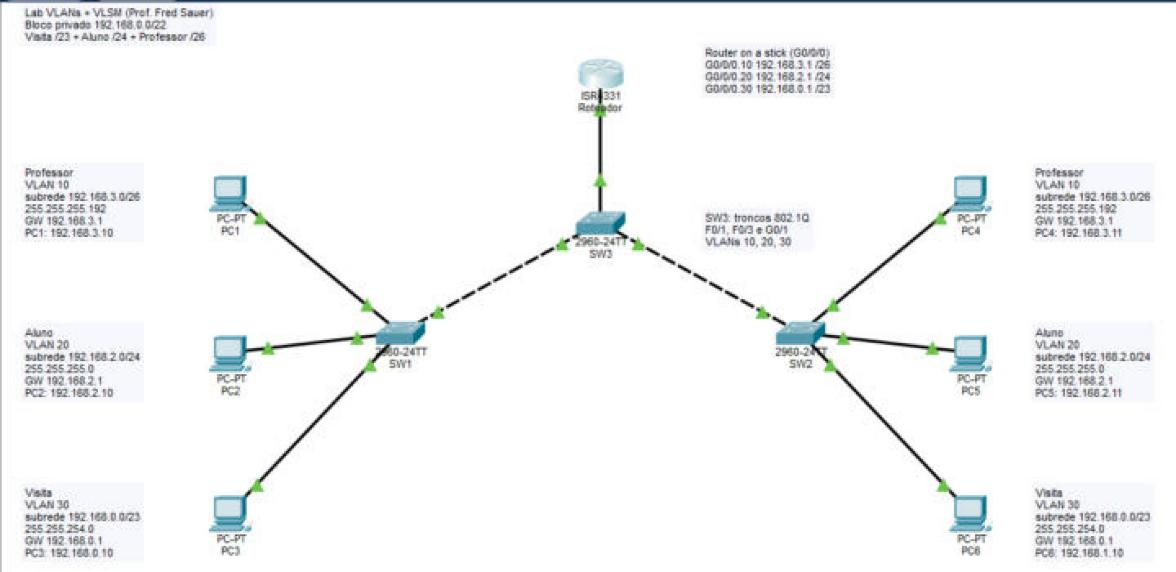
\includegraphics[width=\textwidth]{prints/topologia.png}
\fonteprint
\end{figure}

\subsecao{B.2 Switches}

Nos três switches o \texttt{show vlan brief} lista as VLANs 10 (professor), 20 (aluno) e 30 (visita). No SW1 e no SW2 as portas Fa0/11, Fa0/18 e Fa0/6 aparecem nas suas VLANs, e o \texttt{show interfaces trunk} mostra um tronco em cada um (Fa0/1 no SW1 e Fa0/3 no SW2). No SW3 as VLANs existem sem portas de acesso e os três troncos (Fa0/1, Fa0/3 e Gig0/1) aparecem em modo \emph{on}, com encapsulamento 802.1q, VLAN nativa 1 e somente as VLANs 10, 20 e 30 permitidas.

\begin{figure}[H]
\captionsetup{position=top}
\caption{SW1: show vlan brief e show interfaces trunk}\label{fig:print-sw1}
\centering
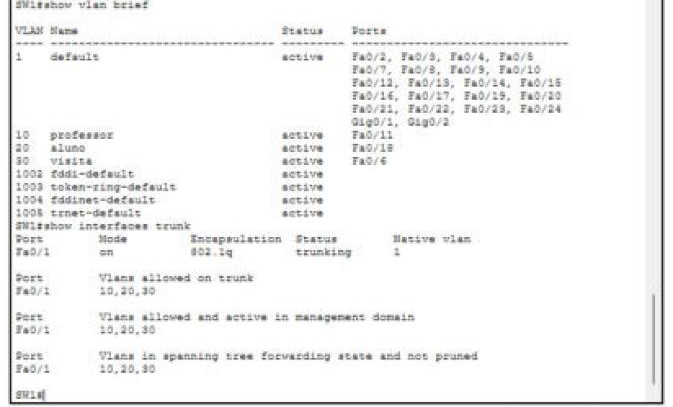
\includegraphics[width=0.70\textwidth]{prints/sw1.png}
\fonteprint
\end{figure}

\begin{figure}[H]
\captionsetup{position=top}
\caption{SW2: show vlan brief e show interfaces trunk}\label{fig:print-sw2}
\centering
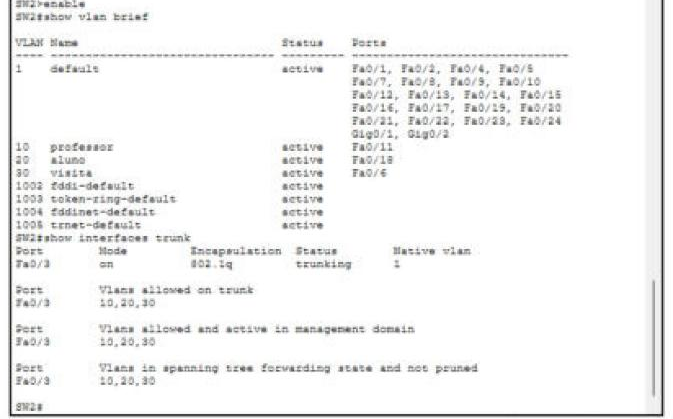
\includegraphics[width=0.70\textwidth]{prints/sw2.png}
\fonteprint
\end{figure}

\begin{figure}[H]
\captionsetup{position=top}
\caption{SW3: show vlan brief e show interfaces trunk}\label{fig:print-sw3}
\centering
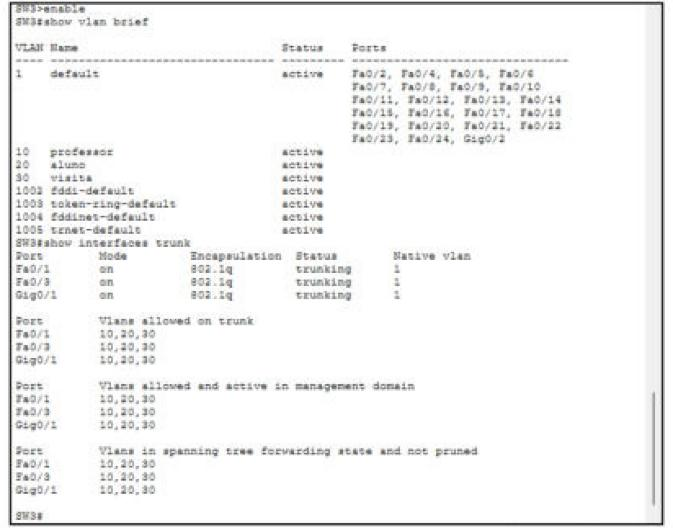
\includegraphics[width=0.70\textwidth]{prints/sw3.png}
\fonteprint
\end{figure}

\subsecao{B.3 Roteador}

O \texttt{show ip interface brief} mostra a G0/0/0 e as três subinterfaces \emph{up/up}, com os IPs dos gateways. O \texttt{show ip route} mostra as três redes diretamente conectadas (192.168.0.0/23, 192.168.2.0/24 e 192.168.3.0/26), cada uma na sua subinterface.

\begin{figure}[H]
\captionsetup{position=top}
\caption{roteador: show ip interface brief e show ip route}\label{fig:print-rot}
\centering
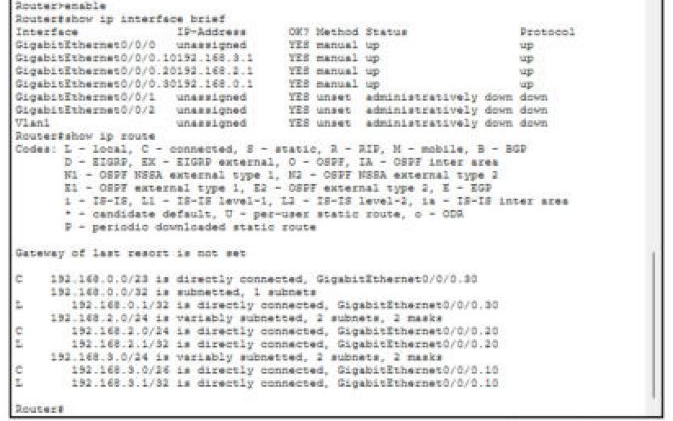
\includegraphics[width=0.78\textwidth]{prints/roteador.png}
\fonteprint
\end{figure}

\subsecao{B.4 Ping e tracert nos PCs}

No PC1 (VLAN 10), o ping para o PC4 (192.168.3.11, mesma VLAN) responde com TTL=128 e o ping para o PC5 (192.168.2.11, VLAN 20) responde com TTL=127, porque passou uma vez pelo roteador. O tracert para o PC5 mostra os dois saltos: o gateway 192.168.3.1 e o destino.

\begin{figure}[H]
\captionsetup{position=top}
\caption{PC1: ping para o PC4, ping para o PC5 e tracert para o PC5}\label{fig:print-pc1}
\centering
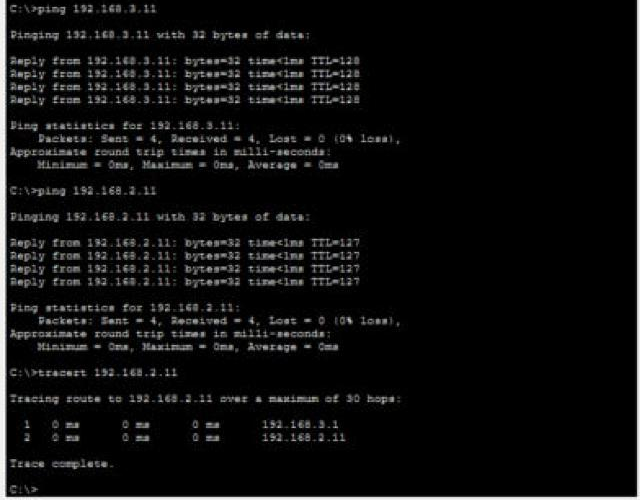
\includegraphics[width=0.62\textwidth]{prints/pc1.png}
\fonteprint
\end{figure}

No PC3 (VLAN 30, 192.168.0.10/23), o tracert para o PC6 (192.168.1.10) tem um salto só, sem passar pelo roteador, embora o 3º octeto seja diferente: os dois estão na mesma /23. O ping para o PC1, que está em outra VLAN, responde com TTL=127.

\begin{figure}[H]
\captionsetup{position=top}
\caption{PC3: ipconfig, tracert para o PC6 e ping para o PC1}\label{fig:print-pc3}
\centering
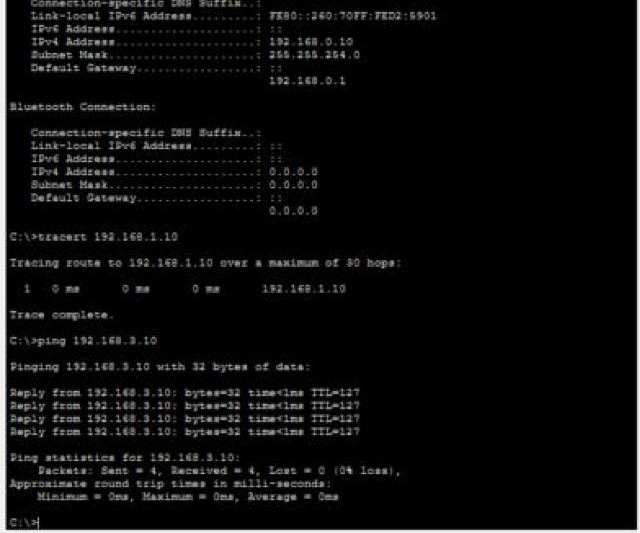
\includegraphics[width=0.62\textwidth]{prints/pc3.png}
\fonteprint
\end{figure}

No PC6 (VLAN 30, 192.168.1.10/23), o tracert para o PC2 (192.168.2.10) passa pelo gateway 192.168.0.1 e chega ao destino. O asterisco na primeira medida do segundo salto é o pacote descartado enquanto o roteador resolvia o MAC do PC2 por ARP. O ping para o próprio gateway responde com TTL=255, o TTL inicial do roteador.

\begin{figure}[H]
\captionsetup{position=top}
\caption{PC6: ipconfig, tracert para o PC2 e ping para o gateway}\label{fig:print-pc6}
\centering
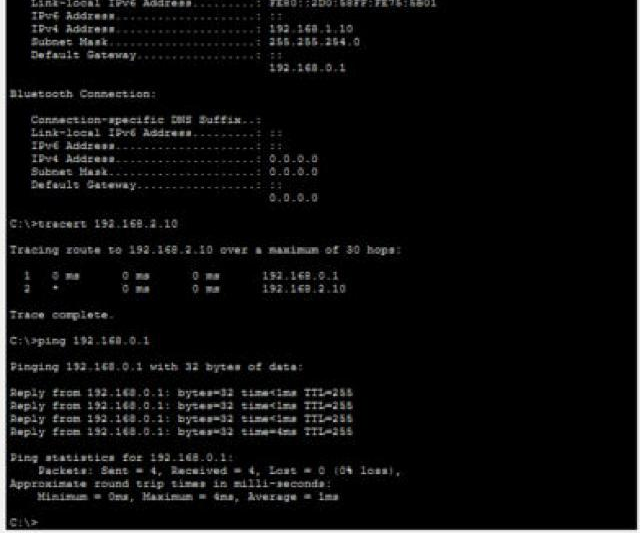
\includegraphics[width=0.62\textwidth]{prints/pc6.png}
\fonteprint
\end{figure}

\subsecao{B.5 Modo simulação}

Com o cenário recém-reiniciado e o filtro em ARP e ICMP, fiz o ping do PC1 para o PC5 no modo simulação. A Figura~\ref{fig:print-sim1} mostra o início da lista de eventos. O broadcast ARP do PC1 passa por SW1, SW3 e SW2 e chega somente ao PC4 e ao roteador, que são os equipamentos da VLAN 10. O primeiro \emph{echo request} vai até o roteador, que então envia o seu ARP na VLAN 20, recebido somente pelo PC2 e pelo PC5.

\begin{figure}[H]
\captionsetup{position=top}
\caption{lista de eventos: ARP do PC1 na VLAN 10 e ARP do roteador na VLAN 20}\label{fig:print-sim1}
\centering
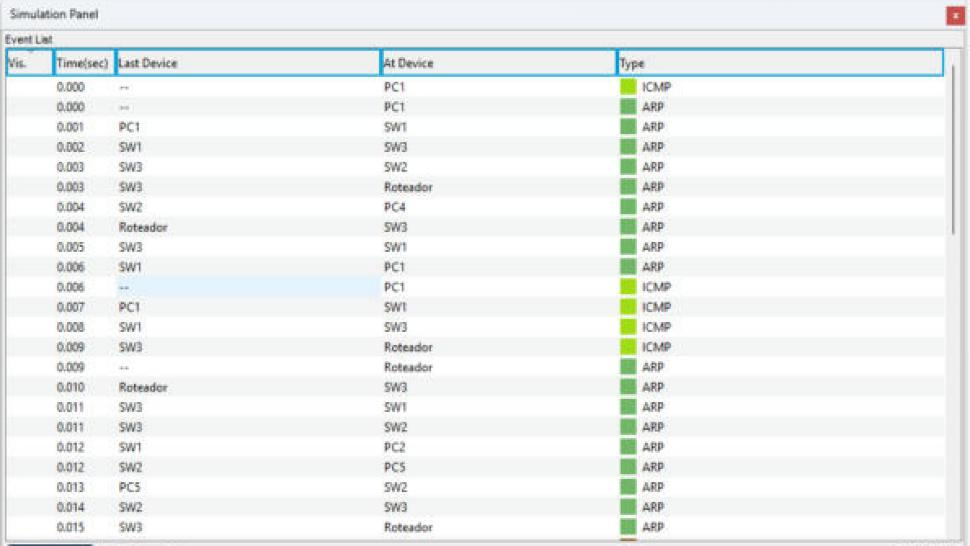
\includegraphics[width=0.88\textwidth]{prints/sim1.png}
\fonteprint
\end{figure}

A Figura~\ref{fig:print-sim2} mostra o segundo ping completo: PC1, SW1, SW3, roteador, SW3, SW2 e PC5 na ida, e o caminho inverso na volta. O pacote passa duas vezes pelo enlace entre o SW3 e o roteador, que é o comportamento do \emph{router on a stick}. Ao fim dos quatro pings o Packet Tracer avisou que o buffer de eventos estava cheio, como o roteiro previa.

\begin{figure}[H]
\captionsetup{position=top}
\caption{lista de eventos: echo request e echo reply passando pelo roteador}\label{fig:print-sim2}
\centering
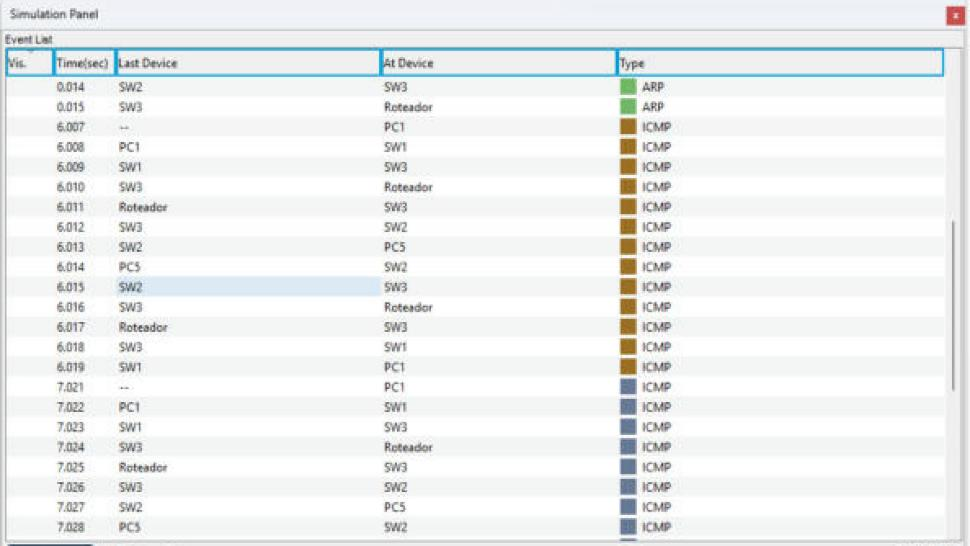
\includegraphics[width=0.88\textwidth]{prints/sim2.png}
\fonteprint
\end{figure}


\vspace{10pt}
{\small Documento construído com LaTeX.}

\end{document}
